\documentclass{article}
\usepackage{graphicx} % Required for inserting images
\usepackage{amsmath}
\usepackage[utf8]{inputenc}
\usepackage[T1]{fontenc}
\usepackage[english]{babel}
\usepackage{geometry}
\usepackage{lmodern}
\geometry{hmargin=2.5cm,vmargin=2.5cm}

% --- Réglages de mise en page ---
\raggedbottom
\widowpenalty=10000
\clubpenalty=10000
\displaywidowpenalty=10000
\setlength{\emergencystretch}{2em}

% --- Pour les blocs de code sémantiques ---
\usepackage{listings}
\usepackage{xcolor}
\usepackage{tikz}
\usetikzlibrary{arrows.meta,positioning,shapes.geometric,fit}

% Configuration des couleurs pour le Turtle / SPARQL
\definecolor{olivegreen}{rgb}{0,0.6,0}
\definecolor{navyblue}{rgb}{0,0,0.5}
\definecolor{mauve}{rgb}{0.58,0,0.82}
\definecolor{lightgray}{gray}{0.95}

\lstdefinelanguage{Turtle}{
    keywords={@prefix,a,owl:Class,owl:ObjectProperty,owl:DatatypeProperty,rdfs:subClassOf,rdfs:domain,rdfs:range,rdfs:label,rdfs:comment,skos:Concept,owl:Ontology,owl:imports},
    keywordstyle=\color{navyblue}\bfseries,
    ndkeywords={fe:,crm:,xsd:,rdfs:,owl:,skos:},
    ndkeywordstyle=\color{mauve}\bfseries,
    identifierstyle=\color{black},
    sensitive=false,
    comment=[l]{\#},
    commentstyle=\color{olivegreen}\italicshape,
    stringstyle=\color{orange},
    morestring=[b]"
}

\lstdefinelanguage{SPARQL}{
    keywords={PREFIX,SELECT,CONSTRUCT,WHERE,VALUES,OPTIONAL,FILTER,
        INSERT,DATA,GRAPH,BIND,AS,DISTINCT,ORDER,BY,LIMIT},
    keywordstyle=\color{navyblue}\bfseries,
    sensitive=false,
    comment=[l]{\#},
    commentstyle=\color{olivegreen}\italicshape,
    stringstyle=\color{orange},
    morestring=[b]"
}

\lstset{
    backgroundcolor=\color{lightgray},
    basicstyle=\ttfamily\small,
    breaklines=true,
    frame=single,
    showstringspaces=false
}
\renewcommand{\lstlistlistingname}{List of Code Listings}

% --- Pour les encadrés stylés du Fil Rouge ---
\usepackage{tcolorbox}
\newtcolorbox{filrouge}{
    colframe=red!75!black,
    title=\textbf{Running Example: The Fort de la Bastille},
    arc=4mm
}

% --- Styles communs des schémas ---
\tikzset{
    schemaBox/.style={
        draw,
        rounded corners=2mm,
        align=center,
        minimum height=9mm,
        text width=3.1cm,
        fill=blue!6
    },
    schemaSmall/.style={
        draw,
        rounded corners=1.5mm,
        align=center,
        minimum height=8mm,
        text width=2.5cm,
        fill=gray!8
    },
    schemaArrow/.style={
        -{Latex[length=2.5mm]},
        thick
    },
    schemaDashed/.style={
        -{Latex[length=2.5mm]},
        thick,
        dashed
    }
}

\title{Design of a Modular Ontology for Crisis Management and Heritage-Site Evacuation Simulation\\[0.4em]
\large Master's Internship Report -- ATLAS Project}
\author{Hugo Poirot}
\date{May 2026}

\begin{document}

\maketitle
\clearpage

\section*{Acknowledgements}
\addcontentsline{toc}{section}{Acknowledgements}

First and foremost, I would like to warmly thank my two internship supervisors, Professor Julie Dugdale and Professor Danielle Ziébelin, for the trust they placed in me and for the quality of their guidance throughout this work.

I am particularly grateful to Julie Dugdale, Professor of Computer Science at Université Grenoble Alpes, researcher at the Grenoble Informatics Laboratory, and head of the SocSIM-K team (\textit{Social Simulation and Knowledge}). Her advice, availability, and expertise in social simulation and crisis management were essential in situating my work within its scientific context. I am also deeply grateful for her encouragement and support as I developed my plans to pursue a PhD.

I also extend my sincere thanks to Danielle Ziébelin, Professor of Computer Science at Université Grenoble Alpes, researcher at the Grenoble Informatics Laboratory within the STEAMER team, and co-director of the Master's programme in Computer Science. Her expertise in knowledge representation, ontologies, and the Semantic Web was invaluable to the design and structuring of the model presented in this report. Her availability, precise feedback, and encouragement in my search for a PhD position greatly contributed to making this internship a defining experience for the next stage of my career.

I would also like to thank Flavien Loup-Hadamard, a PhD candidate in the SocSIM-K team, whose doctoral research provides the main use case for my work. He devoted considerable time to guiding my research, answering my questions, and explaining the scientific and operational challenges of his work on risk and evacuation simulation. Our discussions helped me understand the requirements that the ontology needed to address and grounded my modelling choices in a concrete application.

Finally, I thank all the members of the team for their warm welcome, availability, and the quality of our exchanges throughout the internship. The scientific discussions, technical advice, and various forms of support created a stimulating and supportive working environment. They helped me strengthen my skills, clarify my research interests, and confirm my desire to continue working in knowledge architecture and knowledge representation.

\clearpage

\section*{Abstract}
\addcontentsline{toc}{section}{Abstract}

This internship was carried out within the ATLAS project and the SocSIM-K team at the Grenoble Informatics Laboratory. Its objective was to provide a formal and interoperable representation of the knowledge required to study hazards affecting heritage sites, particularly fires and population evacuation. The resulting contribution is a modular RDF/OWL ontology aligned with CIDOC CRM, complemented by controlled SKOS vocabularies, SHACL constraints, and a prototype data-exchange workflow for a multi-agent system. A declarative evacuation profile selects the classes and properties required by the simulation, drives the generation of SPARQL queries, exports data to a tabular format, and supports the reintegration of simulated results into a provenance-aware historical graph. The architecture separates the domain model, controlled vocabularies, data-quality requirements, and simulator-specific contracts. The deliverable is therefore a reproducible and extensible research prototype whose next stage is validation on a real-world use case.

\textbf{Keywords:} ontology, knowledge graph, RDF, OWL, SKOS, SHACL, CIDOC-CRM, multi-agent system, evacuation, heritage, fire.

\clearpage

\renewcommand{\contentsname}{Table of Contents} % Force the title in French if necessary
\tableofcontents
\clearpage

% --- Liste des figures ---
\listoffigures
\addcontentsline{toc}{section}{List of Figures }
\clearpage

\lstlistoflistings
\addcontentsline{toc}{section} {List of code extracts}
\clearpage

\section*{Introduction}
\addcontentsline{toc}{section} {Introduction }

Faced with the intensification of environmental crises related to climate change, the preservation of cultural and natural heritage sites is a major societal and scientific challenge. The vulnerability of these often composite spaces requires the deployment of highly accurate forecasting and crisis management strategies. It is in this dynamic that the ANR ATLAS (2025--2028) research project, whose ambition is to design a decision support system based on multi-agent simulation to model the spread of risks (such as fires) and optimize evacuation trajectories in complex heritage sites (Thesis under way by Flavien Loup-Hadamard).

The success of such a simulation depends fundamentally on the quality of the representation of knowledge. In fact, a heritage area is not a simple geometric entity: it is a complex socio-ecological system in which physical infrastructures (axes of circulation, buildings), living ecosystems (fauna and flora) and human dynamics (visitors, managers) are articulated. Conventional relational database modelling approaches fail to capture the semantic richness, interoperability of business concepts and flexibility required to cope with highly heterogeneous data, in favour of extreme precision but addressed to specific bodies.

The scientific challenge of this work therefore lies in the use of knowledge engineering as a conceptual bridge between heritage sciences, ecology and simulation computing. The central problem can be formulated as follows: \textit{How to formalize a unified and modular semantic model capable not only of structuring these heterogeneous dimensions, but also of carrying an autonomous inference logic to dynamically quantify the vulnerability of the system? }

This document presents the theoretical and applied contributions made during a six-month research internship with the SocSIM-K team at the Grenoble Informatics Laboratory (LIG). The work focused on designing, developing, and aligning a domain ontology connected to controlled vocabularies through the SKOS standard. Beyond classification alone, the proposed approach provides the foundations for computing heritage, structural, and ecological risk indicators within the semantic knowledge base, thereby avoiding the duplication of domain logic in the simulator.

To describe this approach, the report is structured in five parts. After detailing the institutional framework and research challenges of the project (Part 1), we will quickly go through a state of art of existing projects and models such as the ARCH initiative (Part 2). Part 3 will focus on the modular architecture of ontology developed, illustrating its adherence to the standards of the Semantic Web. We will then detail in Part 4 the semantic inference engine and the translation of the calculation rules into declarative requests. Finally, Part 5 will explore the prospects for the evolution of this model towards modelling the evolutionary dynamics of cultural knowledge.

To make the scientific challenges and abstract modelling choices easier to understand, the report uses a recurring empirical example: the semantic modelling of the Fort de la Bastille in Grenoble. This reference site brings together many of the heterogeneous dimensions addressed by the project. Its rugged Chartreuse topography constrains paths and slopes; its listed fortifications introduce vulnerable historic structures; its peri-urban forests combine biodiversity with combustible biomass; and its population varies considerably between visitors and staff. The Bastille therefore provides a particularly relevant setting in which to assess the robustness of the ontology.
\clearpage
\section{The ATLAS Project and Its Motivation}

\subsection{ATLAS: Preserving Heritage in the Face of Climate Change}

As mentioned earlier, the intensification of the global environmental crisis is increasingly affecting heritage sites around the world. Extreme climatic variations drastically alter their physical conservation conditions, while directly endangering populations, whether in tourist flows or inhabitant communities.

Officially started the \textbf{1 January 2024} for a total of 36 months (ending 31 December 2026), the \textbf{ATLAS} project is a transnational and interdisciplinary collaboration of European scope. The project, funded by the Belmont International Fund (\textit{Belmont Forum}), is financing three national funding agencies: ANR for France, AEI for Spain and MUR for Italy.

The scientific consortium is structured around three core universities: \textit{Universidad Pablo de Olavide} (UPO, Spain), which coordinates the project; \textit{Ca' Foscari University of Venice} (UNIVE, Italy); and \textit{Université Grenoble Alpes} (UGA, France). To validate the digital tools and methodological models developed, ATLAS conducts research and case studies in \textbf{five historic European cities} with diverse geoclimatic settings and vulnerability profiles:
\begin{itemize}
\item \textbf{Seville} and \textbf{Antequera} (Spain) for Mediterranean scenarios and climates;
\item \textbf{Valencia} (Spain) for coastal and heritage dynamics;
\item \textbf{Treviso} (Italy) for the study of continental plains and green infrastructure;
\item \textbf{Grenoble} (France) for vulnerabilities specific to mountain environments.
\end{itemize}

The project's central ambition is to study the relationship between immovable cultural heritage and urban green infrastructure. Although green infrastructure is essential for mitigating urban heat islands and regulating local microclimates, its coexistence with historic buildings also creates complex challenges, including moisture, biological patina, and increased fire risk. ATLAS aims to investigate these interactions using digital technologies.

\subsection{The SocSIM-K Research Team}

The research team \textbf{SocSIM-K} is led by Professor Julie Dugdale, at the Laboratory of Computer Science in Grenoble (LIG). The scientific positioning of the team is at the convergence of the Distributed Artificial Intelligence (IAD), the cognitive sciences and the humanities and social sciences. The fundamental objective of SocSIM-K is to decrypt, formalize and construct computational models of human behaviour within highly complex real environments, in order to simulate their emerging dynamics, explain their causes and improve operational responses in the event of major crises.

\subsubsection{Paradigmatic Foundation: Multi-Agent Social Simulation}

The team's work is fully within the scope of agent-based social simulation. This scientific field is devoted to the study of social phenomena through the prism of multi-agent computer models where each individual, group or institutional component is represented in the form of an autonomous, heterogeneous and intelligent agent.

SocSIM-K's research philosophy is based on a strong multidisciplinary anchor: the conceptualization of behaviours and interactions is not based on purely abstract mathematical assumptions, but is directly based on social science theories and empirical field data. By placing these artificial agents and their decision-making processes within simulated populations, the team seeks in particular to observe how the sum of individual micro-dynamic actions generates macro structures and patterns through a mechanism of emergence.

This use of numerical simulation is essential to explore complex forward-looking scenarios that it would be materially impossible, too expensive, dangerous or ethically unthinkable to experiment in the real world, such as crowd movements in alert situations, managing evacuations from forest fires or sudden floods.

\subsubsection{Research Themes and Cross-Cutting Scientific Challenges}

The team's scientific activity revolves around cardinal keywords: behavioural and cognitive modelling, multi-agent systems, serious games (\textit{serious games}) as well as knowledge engineering, the Semantic Web and the \textit{Linked Data}. It is precisely at the intersection of cognitive modelling and the technologies of the Semantic Web that our internship contributions are located, aimed at formally structuring the knowledge related to historical buildings and their environment.

To carry out its missions, SocSIM-K faces several research challenges and major research challenges:
\begin{itemize}
\item \textbf {The modelling of endogenous factors:} How can we formally translate and inject into the architecture of agents immaterial but predominant variables such as social ties, risk perception, emotions or cognitive biases?
\item \textbf {Cognitive Loyalty:} How can we develop computational models of behaviour that are true representations similar to human decision-making processes in the face of immediate danger?
\item \textbf {Collection and validation:} What methodological protocols collect the initial empirical data, and how can we scientifically validate the robustness of simulators in relation to the real world (especially through crisis exercises or historical data)?
\item \textbf {The transition to scale:} How can we overcome the high computational cost of massive simulations and ensure strict semantic and mathematical consistency in multi-scale simulations?
\end{itemize}

\subsubsection{Application Areas and Convergence with the ATLAS Project}

The expertise of the SocSIM-K team is deployed on a wide range of application areas critical to contemporary society, including pedestrian mobility in urban areas, the impact of environmental factors on cities, analysis of population trajectories, crisis and emergency management, and the preservation and enhancement of cultural heritage.

The contribution of the SocSIM-K team to the ATLAS project is based on a strong historical anchor in the field of crisis modelling, structured by several leading national and international research projects. In particular, the team has developed pioneering expertise through major work on the simulation of large-scale emergencies, such as modelling population behaviour in the face of acute health, seismic or environmental crises. These include contributions from the \textit{ANR CHOUCAS} project (in support of the decision to find victims in the mountains) or active participation in the European project \textit{C2IMPRESS}, which focuses on the co-creative understanding of multi-sea hazards (sudden floods, forest fires).

The ATLAS project therefore does not constitute a break, but the natural extension of this scientific heritage, applied this time to the specific and highly heterogeneous constraints of the cultural and natural heritage in the face of the hazards caused by climate change (floods, fires).

In practice, the team's expertise in human factor modelling, coupled with the need to formalize complex physical infrastructures specific to heritage sites, is the scientific ground upon which the implementation of the simulator under the \textbf{GAMA} platform and the development of our unified semantic model are based. The latter makes it possible to link the vulnerability of physical structures to the behavioural rules of agents in the event of an emergency evacuation.

\subsection{Fire-Evacuation Simulator: Challenges, Specificities, and Requirements}
\label{subsec:simulateur_evacuation_incendie}

The operational implementation of the ANR ATLAS project objectives is based, among other things, on the development of an agent-based fire escape simulator. Such a system can be defined as a computational environment for competing modeling the kinetics of a disaster (flame propagation, temperature rise, smoke opacification of air) and population flow dynamics seeking to escape the danger zone. The aim is to predict displacement trajectories, identify congestion points (bottlenecks) and quantify overall evacuation times in order to test, \textit{in silico}, different crisis management strategies.

\subsubsection{Why Use Simulation in This Context?}

While evacuation simulation is an already proven field for the classical tertiary building (subject to standardized construction standards), its application to a complex socio-ecological and heritage site such as the fort of the Bastille introduces scientific and practical locks that make traditional approaches obsolete, and virtual simulation indispensable:

\begin{enumerate}
\item \textbf {The ethical and material impossibility of real experimentation:} Of course, a real fire cannot be triggered in a protected forest massif or within a fortified structure classified to observe the reactions of the crowd. Similarly, organizing full-scale evacuation exercises across the entire site is extremely complex, costly, and insufficient to reproduce the stress, reduced visibility, or panic factors that affect human behaviour during a real peril.
\item \textbf {The heterogeneity and spatial asymmetry:} Unlike an office building with straight and marked corridors, fort de la Bastille has rugged topography, steep stairs, confined underground boxmates and steep forest hiking trails. The escape axes are intrinsically dependent on the geometry of the site and environmental conditions (a 30 \% slope radically alters the walking speed, and a path can be instantly cut off by a biomass fire).
\item \textbf {Population volatility:} The Bastille welcomes a highly heterogeneous civilian population (foreign tourists, sports hikers, children, people with reduced mobility using the cable car). Their knowledge of the site topography is asymmetrical, and their reactions to the danger cannot be modelled by simple hydraulic flow laws; They require a decision-making engine capable of reflecting this diversity.
\end{enumerate}

\subsubsection{Expected Qualities of the ATLAS Simulator}

To meet the scientific requirements of the project and effectively interconnect with knowledge engineering, the simulator developed (in support of the GAMA platform) must check four basic qualities:

\begin{itemize}
\item \textbf {Cognitive Accuracy:} The simulator should not treat humans as passive physical particles. Agents must be provided with a limited rationality (BDI model), able to perceive their environment imperfectly, communicate with each other, feel stress and change their flight intentions dynamically when their initial route is obstructed.
\item \textbf {Synchronous Multiphysical Coupling:} The simulation engine must have a real-time interaction between fire physics (linear fire front propagation speed, dispersion of toxic gases) and human kinetics. The danger must change the circulation space of the agents (closing of arches of the topological network, reducing the speed of walking due to asphyxiation), and the action of the agents (such as opening or closing of fortified doors) must be able to influence the spread.
\item \textbf {Scenological Flexibility (Scalability):} The architecture should allow site managers to set up and play an infinity of scenarios instantly: vary seasonality (maximum summer vs. winter maintenance), move the starting point of the fire, or test the impact of new emergency signs.
\item \textbf {Semantic Porosity (Ontological Integration):} This is the most critical quality in our work. The simulator shall not function as a black box isolated. He must be able to translate his physical state variables and agents into semantic concepts understandable by our ontology, and vice versa, to question our knowledge base (via declarative requests) to dynamically adapt the behaviour of agents according to the business rules of wealth and risk management.
\end{itemize}

\clearpage
\section{State of the Art}
Semantic modeling of a complex and highly volatile socio-ecological system, such as the Fort de la Bastille, requires the use of proven interoperability standards and the analysis of international initiatives combining heritage and risk management. This section provides a critical overview of ontologies and reference models, cultural data management platforms, as well as major European projects, in order to set the technical milestones for the ATLAS ANR project.
\subsection{The CIDOC CRM Conceptual Reference Model: Foundations and Limitations}
\label{subsec:cidoc_crm_approfondi}

The CIDOC \textit{Conceptual Reference Model} (CRM), formalized by the international standard ISO 21127:2014, represents the culmination of decades of research in knowledge engineering. The primary aim of this high-level ontology is to provide a unified, extensible and formal conceptual framework for the integration, mediation and semantic interoperability of heterogeneous data from museums, archives and libraries.

\subsubsection{An Event-Centred Modelling Approach}

The major paradigm shift introduced by CIDOC-CRM from traditional database architectures (whether relational or object oriented) is its purely event-oriented approach. In classical models, the world is represented statically through rigid entities with direct attributes (e.g., a historic building directly linked to a style or date of construction). This approach fails to capture the transitional and historical nature of heritage knowledge.

On the contrary, CIDOC-CRM postulates that physical entities (\textit{crm:E18\ Physical\ Thing}), actors (\texttt{crm:E39\_Actor}) and abstract concepts (\texttt{crm:E28\_Conceptual\_Object}) do not interact directly, but meet in events (\texttt{crm:E5\_Event}) or activities (\texttt{crm:E7\_Activity}) located in space and time. It is the event that binds entities and bears the semantics of their relationship. This modeling provides an essential flexibility to document the complex life cycles of cultural objects (creation, modification, destruction, change of ownership).

\subsubsection{Core Classes and Extension Mechanisms}

The semantic structure of CIDOC-CRM is based on a network of highly specialized classes and properties. Among the primitives essential for modelling the physical structures of a heritage site are:
\begin{itemize}
\item \textit{crm:E24\ Physical\ Human-Made\ Thing}: This class includes all material creations from human activity. It serves as a root for identifying architectural elements.
\item \textit{crm:E25\ Human-Made\ Feature} : Subclass of the previous, it refers to net physical characteristics which are not isolated objects but which are integrated or grafted into other physical objects (such as fortifications, casemats, doors or traffic axes).
\item \textit{crm:E52\ Time-Span} and \textit{crm:E53\ Place}: These classes allow for geographical and chronological contextualization of events, ensuring rigorous spatial and temporal traceability.
\end{itemize}

One of the challenges for semantic interoperability is solved by using the \textit{crm:E55\ Type} class. Rather than multiplying rigid classes within ontology to specify each trade, CIDOC-CRM delegates fine taxonomy to controlled vocabularies and external thesaurus via the property \textit{crm:P2\ has\ type}. It is this mechanism that allows to associate a SKOS concept (\textit{Structured Thesaurus}) with an OWL class instance, paving the way for modular architectures.

Faced with the need to specialize this general model, the scientific community has developed standardized extensions. The \textit{CRMsci} (\textit{Scientific Observation Model}) is used to formalize scientific measurements and observations, as well as the \textit{CRMarchaeo} dedicated to excavations. More recently, initiatives have emerged to link CIDOC-CRM with geospatial data models such as \textit{GeoSPARQL}, allowing topological properties (\texttt{ogc:geoFlnt}, \texttt{ogc:sfWithin}) to be injected into the cultural graph.

\subsubsection{Structural Limitations with Respect to ATLAS Requirements}

While CIDOC-CRM is an essential standard for heritage management and inventory, critical analysis of its structure reveals fundamental limitations when it comes to exploiting its knowledge in a dynamic crisis simulator such as SocSIM-K:

\begin{enumerate}
\item \textbf {An exclusively descriptive and retrospective nature:} CIDOC-CRM was designed to document the existing one, archive the past and consolidate stable knowledge. It excels in the description of the conservation state or historical provenance of a structure, but is unable to represent transient physical states, variable fluxes or dynamic phenomena in real time.
\item \textbf{Absence of quantifiable physical and mathematical primitives:} The simulation of a hazard (such as a fire) requires the manipulation of explicit physical quantities (thermal conductivity, heat load, rate of siccity of vegetation, linear rate of propagation). CIDOC-CRM has no native property to structure mathematical equations or multiplicative coefficients. The thermophysical and semantic relationships between a composite material and its behaviour in the face of fire do not find a standardized echo.
\item \textbf{Inability to model multiplicative risk and interdependencies: } Within a complex socio-ecological system, vulnerabilities influence each other. For example, the degradation of a forested plant space alters the vulnerability of an adjacent building, which collapses and alters the practicality of a leak axis. CIDOC-CRM does not formalize these complex causal chains and feedback loops natively.
\end{enumerate}

\begin{filrouge}
\textbf{Conceptual application at the Bastille site} \\
By applying the strict CIDOC-CRM standard to the fortifications of the Bastille, the system allows to declare that the host casemate is an instance of \texttt{crm:E25\_Human-Made\_Feature}, typed in \texttt{crm:E55\_Type} as \textit{"Defensive Military Architecture"}. This building can historically be linked to the fortification works of General Haxo via a \texttt{crm:E12\_Production} construction event.

However, in the face of a major fire spreading from the sides of the Chartreuse, the standard model is blind. It is impossible to express semantically that the supporting beams of this casemate have aged, that they have a specific combustibility index, or that the collapse of its roof will generate a source of obstruction (\texttt{fe:BlockingSource}) blocking the only steep trail available to visitors. This lack of physical dynamism justifies the extension and hybridization of the ATLAS model.
\end{filrouge}
\subsection{The European ARCH Project: Resilience Framework and Limits of Transposition}
\label{subsec:arch_project_approfondi}

The European project ARCH (\textit{Advancing Resilience of Historical Areas against Climate-induced and other Hazards}, 2019--2022) is one of the most ambitious attempts at transdisciplinary standardization for assessing and improving the resilience of historic areas to climate and anthropogenic threats. The fundamental contribution of ARCH lies not only in the centralization of technical data, but also in the formalization of a systemic methodological framework, which understands heritage not as an isolated object, but as a complex and interdependent socio-ecological system.

\subsubsection{Technological Architecture and the HArIS System}

At the heart of the ARCH project is the deployment of an ecosystem of interconnected tools, designed to support site managers at all stages of the risk management cycle (analysis \textit{a priori}, real-time monitoring and remediation \textit{a posteriori}). The central pillar of this architecture is the \textit{HARIS} (\textit{Historical Areas Information System}), a rich heritage information system.

The role of HARIS is to go beyond the simple documentary dimension of conventional inventories to store, structure and spatialize multidimensional indicators. Technically, ARCH segmented its analysis around four categories of vulnerability indicators:
\begin{itemize}
\item \textbf {Physical and structural vulnerability:} Intrinsic properties of building materials (sensibility to moisture, mechanical resistance, ageing of envelopes).
\item \textbf {Environmental vulnerability:} Exposure of the site to hazards (frequency of heat peaks, proximity to combustible areas, anthropogenic pressure).
\item \textbf {Socio-economic vulnerability:} Adaptability of local populations, accessibility of relief, use value and tourist attraction.
\item \textbf {Institutional vulnerability:} Existence of backup plans, responsiveness of managers, level of training of maintenance teams.
\end{itemize}

In parallel with HARIS, ARCH integrates the \textit{RMI} (\textit{Resilience Maturity Indicator}), a self-assessment tool to quantify a municipality's maturity level in the face of crises, and a decision support platform to design long-term adaptation strategies.

\subsubsection{Scientific Challenges and Limitations with Respect to ATLAS}

While the conceptual robustness of the ARCH project is indisputable on a macroscopic scale (urban or territorial management), its direct transposition to an operational problem of dynamic crisis management minute per minute (as targeted by the ANR ATLAS project) encounters major research challenges:

\begin{enumerate}
\item \textbf {Macroscopic granularity and the omission of socio-ecological dynamics:} Although the HARIS system of the ARCH project is particularly robust to structure and document the intrinsic vulnerability of the building and heavy infrastructure, it suffers from a major semantic imbalance. It proposes only a very superficial formalisation of the surrounding natural environment (plant biomass, soil water status, biodiversity) and human behavioural factors (crowd dynamics, panic phenomena, mobility profiles).
\item \textbf {The absence of a coupled physical and behavioural simulation engine:} ARCH qualifies the risk (e.g.: \textit{"Zone A exposed to a high fire risk"}) but does not integrate any feedback loop with physical propagation models (thermodynamics, fluid mechanics) or with agent-based models describing human evacuation behaviour. The system detects vulnerability but does not anticipate flight paths in confined or rugged space.
\item \textbf {Semantic partitioning of indicators: } Although ARCH collects multidisciplinary data, they remain siloed within the data model. There is no common semantic scale for interacting an ecological rule (such as nesting a protected species) with a civil infrastructure constraint (the width of an evacuation path) to automatically and inference arbitrate real-time intervention priorities.
\end{enumerate}
\begin{filrouge}
\textbf{Application of ARCH methodology to Bastille} \\
Under the prism of the ARCH project, the Bastille site would undergo extensive qualitative modelling within the HARIS system. The fort would receive indicators of institutional vulnerability (existence of the security plan of the Grenoble metropolis) and socio-economic (massive flows of tourists via the cable car). The fortified building would be assigned a fixed physical vulnerability score, determined by the history of its degradation.

However, should a forest fire of extreme violence be declared on the foothills of the Chartreuse, the ARCH platform would immediately reach its operational limits. It is unable to calculate the biomass ignition index surrounding the casemate, to simulate the progressive asphyxiation of hiking trails by smoke, or to predict how the panic of a school group blocked at the top would alter the accessibility of emergency areas. ARCH provides a strategic compass for long-term adaptation, but leaves the manager with no tactical tool in the face of the immediacy of the peril; It is precisely this conceptual leap, from macro-static to micro-dynamics, that the ATLAS project carries by connecting a simulator.
\end{filrouge}

\subsection{The Arches Heritage-Management Platform: Graph Architecture and Inference Limits}
\label{subsec:arches_platform_approfondi}

Developed jointly by the \textit{Getty Conservation Institute} (GCI) and the \textit{World Monuments Fund} (WMF), \textit {Arches} is a software platform for inventory and management of cultural heritage, distributed under open-source license. Unlike traditional Geographic Information Systems (GIS) or content management software packages disconnected from academic standards, Arches was natively designed to implement Semantic Web technologies and the CIDOC-CRM conceptual reference model. It is one of the most advanced cultural data management tools at the international level.

\subsubsection{Technological Foundations and Entity-Graph Modelling}

Arches' technical originality is based on its ability to mask the intrinsic complexity of semantic description languages (such as OWL or RDF) behind intuitive administration and input interfaces, adapted to heritage experts. Its architecture is based on several fundamental layers:

\begin{itemize}
\item \textbf{Resource Models:} In Arches, each type of heritage entity (a monument, an artifact, an actor, a group) is modelled as a graph oriented of logical entities. These graphs directly translate the CIDOC-CRM property paths. For example, to describe a building, the platform generates a semantic pattern linking a \texttt{crm:E24} root to its subcomponents via standardized relationships, thus guiding the user when entering data.
\item \textbf {Hybrid storage infrastructure:} In the background, Arches pairs the relational and geospatial robustness of \textit{PostgreSQL/PostGIS} for managing complex geometries, to the flexibility and text indexing power of \textit{Elasticsearch}. Semantic resources are stored as JSON-LD documents, allowing polyglot queries combining topological filters and full text semantic searches.
\item \textbf {Terminological management via SKOS:} Arches integrates a concept manager (\textit{Concept Manager}) to import and articulate multilingual business thesaurus to the SKOS standard. Each descriptive node of a resource graph can thus be restricted to controlled values, ensuring perfect homogeneity of cataloguing data.
\end{itemize}

\subsubsection{Conceptual Limitations for Active Simulation}

Despite the elegance of its semantic architecture and its proven efficiency in the national or regional inventory, Arches presents re-defining conceptual locks when it comes to integrating itself as a knowledge engine within an emergency simulation ecosystem such as the ATLAS project:

\begin{enumerate}
\item \textbf {A descriptive and static archiving purpose:} Arches is designed to document memory, monitor the long-term physical macroscopic state of preservation and manage the legal or administrative status of cultural property. Its data model is optimized for human writing transactions and asynchronous consultations. It is absolutely not calibrated to ingest volatile data streams.
\item \textbf {The absence of a semantic reasonmaker and active rule engine:} Although Arches uses the formalism of graphs internally, the platform behaves as a document-oriented database. It does not deploy any active semantic reasonor in the background task (such as a forward chaining inference motor or a description logic processing tool). Arches is able to store the fact that a structure has a given attribute, but it cannot independently deduce new logical triplets (e.g. recalculate a structural hazard index from the thermal degradation of a neighbour) without resorting to heavy third-party application developments outside the graph.
\item \textbf {Resource graph sealing:} In Arches, resource models tend to work in a self-entering manner. Dynamically interacting the graph of a protected plant species with the graph of a fortified building in the form of an environmental impact rule requires complex cross-sectional requests, where a unified ontology nucleus allows a native and fluid semantic porosity.
\end{enumerate}

\begin{filrouge}
\textbf{Application of the Arches platform at the Bastille site} \\
By deploying Arches for the Fort de la Bastille, the conservatives would obtain a tool of remarkable accuracy to catalogue the site at rest. Each casemate and each historical artillery element would have its JSON-LD semantic record aligned with the CIDOC-CRM, while SKOS thesaurus would rigorously specify tree species populate the cliffs of the Chartreuse.

However, if this knowledge base is to be used as an operational emergency decision support tool, the Arches platform is inadequate. It is not structurally designed to receive, store and process dynamic simulation results (such as the progression of a fire front calculated by a physical motor or the evacuation flows of civilian agents). As a result, Arches is unable to directly correlate the hazard sensitivity criteria of its database with volatile environmental data in real time. The platform is able to describe the Bastille statically, but it cannot serve as an interconnected decision-making scoreboard during a crisis. It is precisely to lift this integration lock and allow this convergence between semantic inventory and simulation data that we develop our own modular architecture in Part 3.
\end{filrouge}
\subsection{BDI Social Modelling}

The scope of risk simulation cannot be limited to structural and physical variables alone. The work of the SocSIM-K team provides a convincing illustration of this, placing human behaviour in crisis situations at the heart of its major research areas. Therefore, the understanding of contemporary tools dedicated to the representation of the human factor is indispensable. This need justifies the study of the \emph{Beliefs-Desires-Intentions} (BDI) model, which is now the benchmark for multi-agent social simulation.

\subsubsection{Architecture and Formalism }

The architecture of the BDI model has an apparent simplicity, with its robustness based mainly on a dynamic circular-linked inference system. This computational structure is broken down into three conceptual layers:

\begin{itemize}
\item[\textbf{Beliefs (Beliefs):}] This set represents the informational state of the agent, that is, his perception of his environment. These beliefs incorporate rules of inference that allow, by chaining before, to generate new beliefs. The term "belief" is preferred here to that of "knowledge", as this information may be erroneous or outdated. This first level acts as a filter on observable data by assigning a specific weight to them.
    
\item[\textbf{Desires (Désirs):}] They characterize the motivational state of the agent by defining the objectives or situations he wishes to accomplish or provoke. A distinction must be made between desires and operational objectives, which correspond to the desires "for which the agent engages in active pursuit". This set plays a major role in the inference and deliberation phases.
    
\item[\textbf{Intentions (Intentions):}] They embody the deliberative state of the agent and can be defined as operationalized desires associated with action plans. A plan consists of a sequence of actions that the agent is likely to carry out to realize his intentions. Because of their potentially interlocking structure, these plans are initially designed in a partial manner. Their gradual completion over the course of execution gives the model all its relevance: plans remain continually influenced by beliefs and desires, while retroacting to them as they are realized.
\end{itemize}
\subsubsection{Operational Dynamics: Events and the Reasoning Cycle}

The movement of this cognitive architecture is based on a software execution loop, dictated by the treatment of ecosystems of** events** and mechanisms of**inference**. Events act as the fundamental catalysts of agent dynamics. They are structured into two categories:

\begin{enumerate}
\item \textbf {External events:} Generated by the physical environment of the simulation, they are perceived by the agent via its sensors. These events trigger an immediate update of the belief base (\textit{Belief Revision Function}) and may force the agent to modify an ongoing plan that has become obsolete or dangerous.
\item \textbf {Internal events:} Generated autonomously by the agent himself during his cycle of deliberation, they materialize changes in psychological states. For example, the emergence of a new belief may lead internally to the emergence of a new sub-objective, or the failure of an action within a plan may trigger an internal retreat event to force the evaluation of an alternative plan.
\end{enumerate}

The computational heart of the BDI agent lies in its ability to orchestrate these event flows through its inference loop. With each iteration, the reasoning engine confronts the events received with the existing beliefs to bring out new options (generation of desires). The deliberation process then selects the best options, which become intentions, and then a planning mechanism combines with these intentions the appropriate action plans extracted from the officer's plan library.

This architecture provides a critical balance between \textit{proactivity} (the agent pursues its objectives persistently through its intentions) and \textit{reactivity} (external events allow it to adapt instantly to the ruptures of its environment).
\subsubsection{Connection with ATLAS: Rationale and Semantic Synergy}

The integration of the BDI model at the heart of the ANR ATLAS project is not simply an opportunistic technical choice, but directly responds to a major research challenge in the project: the need to simulate human evacuation behaviour that is both realistic, heterogeneous and dynamic in the face of a sudden peril. Conventional simulation approaches (particular or cellular automaton models) often treat individuals as homogeneous physical entities subject to mechanical attraction or repulsion forces. However, in a composite and rugged space such as the fort of the Bastille, the decision to flee is intrinsically linked to the cognitive perception, knowledge and psychological bias of each individual.

The BDI model is the ideal paradigm for the ATLAS project for three fundamental reasons:

\begin{enumerate}
\item \textbf {Management of limited and asymmetrical rationality:} During a fire on the sides of the Chartreuse, a tourist who discovers the fort for the first time will not have the same perception of space, nor the same reflexes, as a cable car maintenance agent. The formalism of BDI allows for the creation of differentiated agent profiles. Their bases of \textit {Beliefs} initials will be asymmetrical, which will condition the relevance of their \textit{Intentions} and the success of their evacuation trajectories.
\item \textbf {Direct coupling with ontology:} This is where the major point of articulation of our work is located. Traditionally, the beliefs of a BDI agent are mandatoryly coded within the simulator. The objective of our work within the project is to propose an approach where **the basis of Officer Belief is directly fed and semantically structured by our high-level ontology**. The physical environment of the fort, the SKOS thesaurus characterizing the types of danger, and the rules of inference developed in Part 4 become the agent's conceptual reading grid. The knowledge graph is thus inserted as the formal support of the perception of the agent.
\item \textbf {The dynamicity of feedback loops:} A crisis simulator must model the unexpected. The BDI reasoning cycle excels in the management of ruptures. When a semantic rule deduced by our inference engine describes a path as "impracticable", this information is pushed as an external event in the loop of the agent's reasonmaker. The impact is immediate: the agent re-evaluates his options, takes his current action plan and reconstructs a new one, thus reproducing the mechanisms of rehabilitation and human panic in real time.
\end{enumerate}

In short, the BDI model provides the human decision-making engine, by connecting this paradigm to the ATLAS project, it provides a framework capable of simulating not only the physical propagation of a hazard, but also the psychological and behavioural spread of the crisis within the population of the site.
\begin{filrouge}
\textbf{Application of the BDI model at the Bastille site} \\
Applied to visitor flows on the Bastille site, the BDI model simulates realistic and non-mechanical evacuation behaviour. Imagine a visitor located at the top terraces of the Bastille when the fire breaks out.

Its initial state includes the \textbf{croyance} that the only means of rapid descent is the cable car. The appearance of a major \textbf{external event}, the technical shutdown of the cable car due to smoke, updates his beliefs. This rupture generates an emergency \textbf{internal event} that modifies its \textbf{desirs} (the absolute priority becomes the leak on foot) and reconfigures its \textbf{intentions}: descend through the stairs of the east slope. The agent then extracts a topological action plan from his memory.

If, during his descent, a new external event tells him that the chosen path is saturated by a panic crowd, his loop of inference will re-evaluate his beliefs in real time, abandon the current intention, and autonomously bifurcate towards an alternative plan (go back to the fortified casemates). It is this coupling between the cognitive flexibility of the BDI model for humans and the richness of ontology for physical structures that characterizes the contribution of the ATLAS project.
\end{filrouge}

\subsection{The GAMA Simulation Platform: Agent Environment and Semantic Integration}
\label{subsec:plateforme_gama}

The theoretical formalization of human behaviour via the BDI model cannot be achieved without a computational execution medium capable of managing the spatial complexity and asynchronism of agents. As part of the research carried out within the SocSIM-K team for the ANR ATLAS project, and in direct support of the development of Flavien Loup-Hadamard's thesis, the technological choice focused on the platform \textit{GAMA} (\textit{GIS Agent-based Modeling Architecture}). This open-source modelling and simulation environment is required as an academic standard for the manipulation of large-scale complex multi-agent systems, particularly due to its native capacities for coupling between spatial dynamics and cognitive architectures.

\subsubsection{Native Support for Geospatial Data and BDI}

GAMA's main asset lies in its ability to unify two dimensions that are often partitioned in traditional simulators: advanced spatial analysis (SIG) and cognitive modelling of agents.

On the one hand, GAMA integrates a vector geospatial layer and raster high level. Unlike platforms like NetLogo, where space is discretized into a rigid cell grid (\textit{patches}), GAMA allows agents to evolve in a continuous topological environment, directly imported from form files (\textit{Shapefiles}GIS) or OpenStreetMap data. Complex geometries (building polygons, traffic axis lines) become full agents or strict spatial constraints governing movement.

On the other hand, GAMA natively embarks since its recent versions a full implementation of the BDI architecture via its dedicated language, the GAML (\textit{GAma Modeling Language}). This software integration allows the modeler to explicitly declare predicates of beliefs, desires and intentions of agents, as well as structures of reflexive plans or belief revision functions, without having to manipulate heavy third-party libraries in Java.

\subsubsection{The Dynamicity Challenge: Events and Semantic Coupling}

At the heart of the simulator, the GAMA execution cycle orchestrates the dynamicity of the system through fine event management. At each step of time (\textit{simulation step}), the platform updates the physical environment, for example, the spatial-temporal progression of a fire front simulated by propagation equations, and propagates these changes as stimuli to the agents. GAMA manages natively:
\begin{itemize}
\item \textbf {Active and passive perception:} Agents inspect their geospatial neighbourhoods using a cone of vision or a defined perception radius, transforming the physical attributes of space into external events that feed their BDI loop.
\item \textbf {The generation of internal events:} The failure of a displacement or completion of a space objective instantly generates internal signals within the GAML engine, forcing the agent to recalculate a route or modify its motivational priorities.
\end{itemize}

However, the scientific lock lies in the nature of this knowledge. If GAMA excels in executing the behavioral logic minute per minute, its internal structure remains optimized for imperative data structures. This is where alignment with our ontology takes on its full meaning: the challenge is to go beyond the simple local variables of GAMA to index the beliefs of the agents on the standardized concepts of our semantic graph, allowing a deported and interoperable reasoning.

\begin{filrouge}
\textbf{Application of the GAMA platform at the Bastille site} \\
In the ATLAS simulation developed by F. Loup-Hadamard, the Fort de la Bastille is instantiated in GAMA from real elevation and vector data describing the Grenoble terrain. The steep Chartreuse paths and casemate stairways are converted into a topological circulation network in which slope directly affects agent walking speed.

When a virtual fire is initialized on the slope, GAMA calculates the spread of the hazard. If a "Visitor" agent, with a BDI architecture under GAML, is on Guy Pape's prairie path, his perception function captures the external event "smoke presence" on the network arc he was about to take. The GAMA BDI engine immediately suspends the current running plan.

Thanks to the semantic interconnection that we propose, the agent describes this perception not as a simple boolean variable isolated, but as an instance of disturbance linked to the concepts of vulnerability of our ontology, allowing it to deduce, via the inference engine, that the axis has become impracticable and that it must initiate a retreat path towards the upper station of the cable car.
\end{filrouge}
\subsection{Conclusion: Summary of ATLAS Technical Requirements and Research Challenges}
\label{subsec:conclusion_besoins_techniques}

The cross-critical analysis of Semantics Web standards and international heritage management platforms highlights a major technological gap. On the one hand, the CIDOC-CRM and the Arches platform offer a descriptive semantic frame with remarkable precision to catalogue heritage in a static and retrospective way. On the other hand, systemic initiatives such as the ARCH project formalize macroscopic indicators of resilience, but fail to interconnect them in a fine and dynamic way with the natural environment and human flows.

The ANR ATLAS project is part of the convergence of these approaches to lift these challenges. To transform a passive inventory into a truly multi-criteria and multi-hazard decision support (DSS) system, four imperative technical needs guide our work:

\begin{enumerate}
\item \textbf {Semantic unification by an Ontology Modular Core:} It is essential to overcome the partitioning of data by designing an extension of the CIDOC-CRM capable of dialogue within a single graph of ontologies of radically heterogeneous domains. Physical infrastructure (buildings, roads), the natural ecosystem (plant biomass, wildlife) and the population must share a common semantic metamodel.
\item \textbf {Standardization and comparability of vulnerability indicators:} In order to effectively guide arbitration in a crisis, risks of totally different nature (the risk of collapse of a historical masonry, the risk of undergrowth and the panic threshold of a crowd) must be translated and standardized on a common and comparable semantic vulnerability scale.
\item \textbf{Use of declarative logic and an externalised inference engine:} To preserve scalability and interoperability, complex vulnerability indicators should not be hard-coded in external imperative scripts. Domain logic should instead be expressed declaratively through the knowledge base, inference rules, and constructive SPARQL queries capable of deriving new vulnerability statements.
\item \textbf {Asynchronous interconnection with Multi-Agent Simulator:} Architecture must be designed to serve as a bridge for integration. Without attempting to simulate physical or behavioural dynamics itself, ontology must be able to receive, correlate and structure the results of the evacuation simulator developed by the \textit{SocSIM-K} team and fire propagation models, thus acting as the semantic decision-making core of the global system.
\end{enumerate}

\begin{filrouge}
\textbf {From state of art to active architecture for the Bastille} \\
In summary, the state of the art shows us that in the face of a fire threatening the Bastille site, the existing tools remain unarmed: the CIDOC-CRM will describe the history of the casemate, ARCH will give an overall risk note to the metropolis, and Arches will display a frozen technical sheet of fortifications. None is able to correlate the fact that the dryness of the Chartreuse forest (environmental data) increases the thermal vulnerability of the casemate's beams, and that the collapse of the casemate (physical simulation result) will obstruct the only path that can be followed by the school group during evacuation (behavioral simulation result).

The architecture of our ontology was designed to fill this gap in interconnection and correlation. The technical needs thus identified trace the roadmap of the following sections of this report: the formalization of our unified modular structure (Part 3), followed by the implementation of its logic of inference and its query mechanisms for decision support (Part 4).
\end{filrouge}
\clearpage

\section{The FE Ontology}
In this section, we will present the conceptual and operational interests of creating an ontology of the representation of heritage sites and the risks that threaten them. In this case we begin with a general approach to the concept of ontology and its technical specificity. We will then detail the technological choices made and the reasons for them. Once the technical bases have been laid out, we will end this part with a more detailed presentation of the current form of ontology, in particular to put its finesse without loss of versatility.

\subsection{Objectives and Benefits of Ontological Modelling}

In computer science, formal representation of knowledge is a fundamental challenge. Although the relational model remains the dominant standard due to its maturity and transactional efficiency, it is structurally limited as the field of study becomes more complex. As part of our work, although pre-existing relational databases — like the ARCH database — ensure the persistence of primary data, they struggle to capture the richness of semantic interconnections between anthropogenic and environmental factors influencing our subject matter.

To overcome these limitations, the shift from storage-based modelling (SGBD) to knowledge-based modelling (ontology) is essential. Unlike standard graph-oriented models, ontology is not limited to mapping entities and their relationships; It creates a layer of upper abstraction based on formal representational languages (such as OWL or RDF). This structure is structured around three pillars:
\begin{enumerate}
\item \textbf {Taxonomy and semantics:} A rigorous definition of classes, inheritance hierarchies and properties (roles) between objects.
\item \textbf {Coherence control:} Application of logical constraints (cardiality, domains and ranges of values) guaranteeing model integrity.
\item \textbf {Conceptual Inference:} Using chaining axioms that allow automatic reasoners to deduce implicit relationships, thus promoting the emergence of new knowledge without weighing down the physical structure of the graph.
\end{enumerate}

In view of the requirements of the ATLAS project, the relational model, by its rigid nature and static typing, appears insufficient to understand the transversality of heritage sites and the dynamics of their conservation. Moreover, the challenge of interoperability within the entire research work of the project requires an architecture capable of transcending data silos. The adoption of an ontological approach solves several structural blockages:

\begin{itemize}
\item \textbf{Interoperability and Semantic Alignment:} Ontology allows semantics to be decoupled from the concepts of their linguistic labelling. By aligning with standards such as CIDOC-CRM, it becomes possible to interconnect heterogeneous data sets, thus resolving the language gap inherent in international collaborations.
\item \textbf {Flexibility and evolutionary extensibility:} Contrary to the rigidity of relational patterns, where each modification requires a complex restructuring of tables (and associated joints), the ontological model allows an incremental extension. The addition of new concepts or properties is done by simply enriching the graph without altering the consistency of existing data.
\item \textbf{Analytical power and reasoning:} Integrating reasoners supports both visual graph exploration and the execution of complex semantic queries. Dynamic navigation through the graph turns the system into a scientific discovery tool capable of revealing correlations that would be difficult to express through conventional SQL queries.
\item \textbf {Adaptive Granularity:} Through modularisation mechanisms and the use of controlled vocabularies, the model allows for "local specialization". Each partner can maintain a specific business granularity, while ensuring top-down interoperability with the overall project benchmark, thus ensuring the long-term sustainability and coherence of the architecture.
\end{itemize}

\subsection{RDF Triples: The Elementary Building Blocks of Knowledge}

In the Semantic Web ecosystem, the representation of knowledge is based on a fundamental paradigm: the decomposition of any information into atomic units called \textit{triplets RDF} (Resource Description Framework). Unlike traditional data models, which lock attributes into rigid tables, the RDF model offers a decentralized relational structure based on the triad: \textbf{Subject – Predicate – Object}.

\subsubsection{Anatomy of a Triple}
Each fact within our ontology is articulated according to this logical pattern:
\begin{itemize}
\item \textbf{Subject:} It represents the source entity, the main node of the graph. In the context of our project, for example, it is a specific "building" body.
\item \textbf{The Predicate:} It defines the nature of the relationship or property that unites the subject with the object. This predicate acts as a oriented arc connecting the two entities.
\item \textbf {Object:} It is the target of the relationship. The object may be either another entity (e.g. a "Geographical Area"), or a literal value (e.g. a data typed as an integer or a string of characters).
\end{itemize}

This model imposes a major conceptual break: the data is no longer a static property encapsulated in an object (like classical object-oriented programming), but a dynamic relationship. For example, the height of a monument is not an internal attribute, but the result of a triplet linking the building to a decimal value via a specific measuring property. This approach allows metadata and topological relationships to be treated uniformly. Figure~\ref{fig:rdf-triplet} illustrates this elemental decomposition.

\begin{figure}[htbp]
\centering
    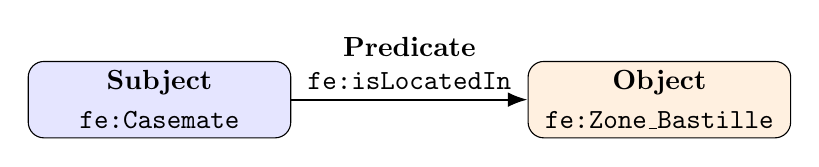
\begin{tikzpicture}[node distance=3cm]
        \node[schemaBox,fill=blue!10] (subject) {\textbf{Subject}\\[0.2em]\texttt{fe:Casemate}};
        \node[schemaBox,fill=orange!12,right=of subject] (object) {\textbf{Object}\\[0.2em]\texttt{fe:Zone\_Bastille}};
        \draw[schemaArrow] (subject) -- node[above,align=center] {\textbf{Predicate}\\\texttt{fe:isLocatedIn}} (object);
    \end{tikzpicture}
\caption{Representation of a statement as an RDF triple}
\label{fig:rdf-triplet}
\end{figure}


\subsubsection {The power of taxonomy and inheritance }
Beyond the assertion of individual facts, an ontology derives much of its expressive power from class hierarchies. Entities are organised within taxonomies that support inheritance. When a class is defined as a subclass of another---for example, when \textit{Building} is a subclass of \textit{Physical Object}---it inherits the semantic commitments associated with its parent class.

This architecture offers two key benefits for the sustainability of the project:
\begin{enumerate}
\item \textbf{Elimination of redundancy:} There is no need to redefine, for each type of entity, universal properties such as creation date or spatial location. By inheriting generic classes, our objects retain a coherent and lightweight structure.
\item \textbf{Enhanced interoperability:} This structure allows third-party users and systems to query complex data without knowing every internal specialisation. A query concerning physical entities can also return buildings through subclass reasoning, thereby supporting consistent access across the dataset.
\end{enumerate}

Finally, although standards such as CIDOC-CRM offer extensive vocabulary, ontology retains total flexibility. It is possible to define new specialized properties to meet the emerging needs of the field. This extensibility makes it possible to refine the representation without ever compromising the compatibility with international standards, thus ensuring that the ATLAS project remains open to future research developments.
\subsubsection {The semantics of properties: beyond the simple relationship}

In an ontology, properties are not merely channels for carrying information; they are first-class elements with formal logical semantics. Unlike a relational join, an RDF/OWL predicate specifies how a relationship is interpreted by reasoning engines.

\paragraph{Typology and logical behavior }
The definition of a property is accompanied by a typing that enriches the inference capacity of the system:

\begin{itemize}
\item \textbf{Transitive properties:} They allow the spread of the relationship through a chain of objects. If a $P$ property is transitive, then the $A \xrightarrow{P} B$ and $B \xrightarrow{P} C$ relationship necessarily implies $A \xrightarrow{P} C$. This is crucial for modeling geographic hierarchies: if the \textit{Site A} is located in the \textit{Zone B}, and the \textit{Zone B} is located in the \textit{Region C}, then the system automatically deduces that the \textit{Site A} is located in the \textit{Region C}.
    
\item \textbf{Symmetric properties:} A property is symmetric when a relation from subject $S$ to object $O$ also entails the same relation from $O$ to $S$. An adjacency property is a typical example. A single assertion is therefore sufficient for the reasoner to derive both directions.

\item \textbf{Inverse properties:} This mechanism allows for the establishment of reciprocal relations between two distinct predicates. For example, if we define \textit{aForarchitecture} as the opposite of \textit{aDesigned}, the system becomes able to deduce all buildings designed by a given architect from the simple list of architects associated with the buildings. This duality offers exceptional request flexibility.
\end{itemize}



\paragraph{Domains and Ranges of Values }
To ensure semantic consistency, each property is constrained by its \textbf{domain} (the type of subject it accepts) and its \textbf{plage of values} (the type of object it can connect).

This configuration acts as a real-time validation filter:
\begin{enumerate}
\item \textbf {The Domain} defines all classes for which the property is valid. If a \textit{aPourHauteur} property has the \textit{Building} as its domain, attempting to apply this property to a \textit{People} class will trigger a consistency alert.
\item \textbf {The Range of Values (Range)} restricts the type of target. For example, a \textit{locatedIn} property will have the \textit{Geographical Area} as its range.
\end{enumerate}

This logical rigour is what allows ontologies to go beyond simple storage to become tools of \textit{semantic verification}. The system becomes able to detect inconsistencies that would remain invisible in a classical relational scheme, because it does not just store the data, it "understands" the validity of the fact expressed according to the defined axioms. This layer of implicit knowledge, generated by the very nature of the properties, transforms each database into a graph capable of self-validation and automatic enrichment.
\subsection{Skos Vocabulary}

The design of ontology quickly revealed a necessary distinction between the stable structure of the domain and the values used to classify entities. An OWL class represents a category of objects with its own structure, properties and possibly constraints. Conversely, a value such as a type of axis, a population category, a plant species or a level of accessibility is more part of a repository that can evolve with the uses and partners of the project. These values were therefore organized in the form of vocabularies controlled by the SKOS standard (\textit{Simple Knowledge Organization System}).

SKOS allows you to define concepts, bring them together in conceptual diagrams and associate them with preferential wording, synonyms, documentary notes or hierarchical relationships. This organization responds directly to the international and multidisciplinary nature of ATLAS. The same concept may have several linguistic representations without changing its identifier or its computer significance. The simulator code, a SPARQL request, and a Francophone or Anglophone user can refer to a common resource.

In the deliverable, thesaurus is separated by domain: hazards, artifacts, axes, buildings, cognitive factors, natural spaces, species, heritage sites, impacts, populations, security, victims, weather and areas. This separation reproduces the modularity of OWL ontology and avoids concentrating all values in a monolithic repository. Each SKOS concept is linked to a classification class defined by ontology. Ontology therefore retains the meaning of the relationship, while the thesaurus provides the authorized values and their terminology organization.

The modeling rule is as follows: a concept becomes an OWL class when it has to carry its own properties, participate in structuring relationships, be targeted by a constraint or play an autonomous role in simulation. It becomes a SKOS concept when it is primarily a classification value. Thus, a traffic axis is a class because it has a length, width, capacity and connections. On the other hand, \textit{series}, \textit{shall} or \textit{shall} are concepts likely to type an axis.

\begin{lstlisting}[language=Turtle,caption={Example of a controlled concept in a SKOS thesaurus}]
fe:Fire a skos:Concept, fe:HazardType ;
    skos:prefLabel "Incendie"@fr ;
    skos:prefLabel "Fire"@en ;
    skos:inScheme fe:HazardTaxonomy .
\end{lstlisting}

Finally, this separation is important for maintenance. The addition of a new species, new material or a new type of hazard does not require a systematic modification of the OWL structure. Specialists can enrich vocabulary without questioning the classes and properties already used by other modules. Also, this organization allows to reuse thesaurus in other projects, even if the structure of ontology changes. SKOS concepts are thus more easily shared and interoperable than OWL classes. At the same time, this ensures that the history of the simulation versions is maintained, since the SKOS concepts can be aligned with specific versions of OWL ontology.

\subsection{Schema Selected }

The selected architecture is based on four complementary layers. The first is the RDF/OWL model, which describes the domain entities and their relationships. The second is the SKOS thesaurus, which carries the controlled values. The third uses SHACL to express the quality constraints applicable to the data, ensuring the consistency of the data. The fourth consists of reporting profiles describing the specific needs of a multi-agent system. This separation avoids confusing domain knowledge, terminology, validation and the requirements of a particular application.

The ontology entry point is the \texttt{fe\_core.ttl} module. It contains shared abstractions and imports thematic modules. Responsibility is distributed among sites, areas, buildings, axes, populations, cognitive factors, hazards and safety, impacts, weather, natural spaces, artifacts, victims and simulation. When a concept concerns several domains, it is placed in the module carrying its main entity and then linked to others by properties. This organization limits duplications and allows an incremental evolution of the model.

Project-specific classes are aligned, where relevant, with CIDOC-CRM categories. Physical objects and entities are reconciled to classes such as \texttt{crm:E18\_Physical\_Thing}, \texttt{crm:E25\_Man\_Made\_Feature} or \texttt{crm:E70\_Thing}. The materials are attached to \texttt{crm:E57\_Material}, the types to \texttt{crm:E55\_Type}, the dimensions to \texttt{crm:E54\_Dimension}, the states to \texttt{crm:E3\_Condition\_State} and the simulation activities to \texttt{crm:E7\_Activity}. Ontology FE therefore does not replace the heritage reference model: it specializes in representing knowledge specific to hazards, evacuations and simulations.

SHACL constraints occupy a distinct place in this diagram. The open world of RDF naturally allows incomplete graphs: the absence of a property does not mean that it is false. However, a simulator cannot function if an indispensable data, such as the length of an axis or the size of a population, is missing at its entry. SHACL allows us to express these obligations without turning them into universal truths of ontology. The repository thus contains general constraints per domain and a specialized form for MAS evacuation entrances. Figure~\ref{fig:semantic-architecture} summarizes the division of responsibilities between the four layers.

\begin{lstlisting}[language=Turtle,caption={Module import principle from FE kernel}]
fe:CoreOntology a owl:Ontology ;
    owl:imports
        fe:SiteOntology,
        fe:ZoneOntology,
        fe:BuildingOntology,
        fe:AxisOntology,
        fe:PopulationOntology,
        fe:HazardAndSafetyOntology,
        fe:SimulationOntology .
\end{lstlisting}

\begin{figure}[htbp]
\centering
\resizebox{0.96\textwidth}{! } {
    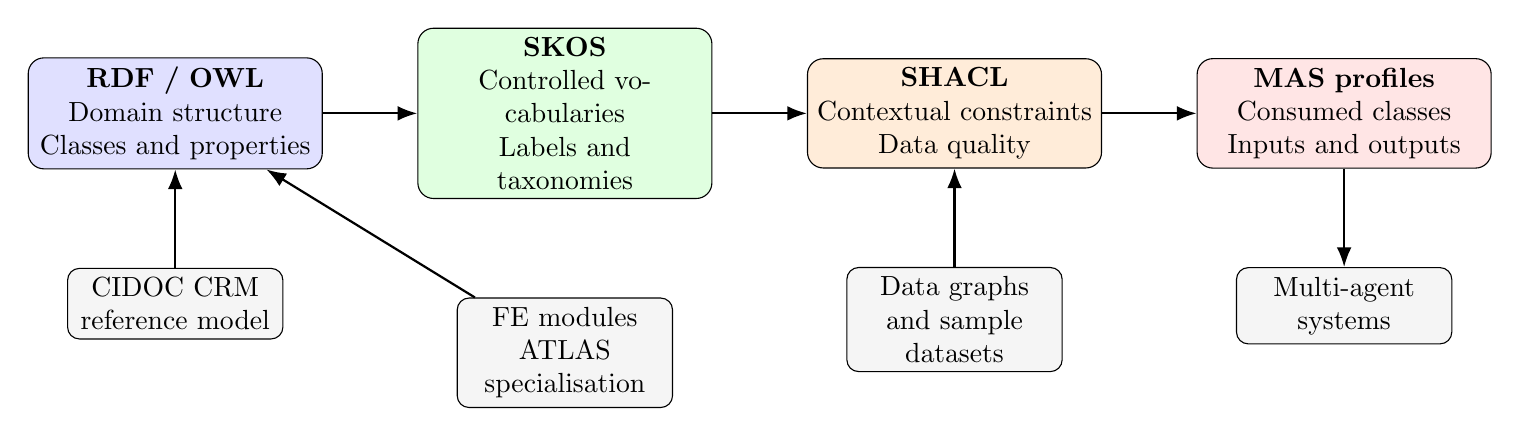
\begin{tikzpicture}[node distance=1.1cm and 1.2cm]
        \node[schemaBox,fill=blue!12,text width=3.5cm] (owl) {\textbf{RDF / OWL}\\Domain structure\\Classes and properties};
        \node[schemaBox,fill=green!12,text width=3.5cm,right=of owl] (skos) {\textbf{SKOS}\\Controlled vocabularies\\Labels and taxonomies};
        \node[schemaBox,fill=orange!15,text width=3.5cm,right=of skos] (shacl) {\textbf{SHACL}\\Contextual constraints\\Data quality};
        \node[schemaBox,fill=red!10,text width=3.5cm,right=of shacl] (profile) {\textbf{MAS profiles}\\Consumed classes\\Inputs and outputs};

        \draw[schemaArrow] (owl) -- (skos);
        \draw[schemaArrow] (skos) -- (shacl);
        \draw[schemaArrow] (shacl) -- (profile);

        \node[schemaSmall,below=1.25cm of owl] (crm) {CIDOC CRM\\reference model};
        \node[schemaSmall,below=1.25cm of skos] (modules) {FE modules\\ATLAS specialisation};
        \node[schemaSmall,below=1.25cm of shacl] (data) {Data graphs\\and sample datasets};
        \node[schemaSmall,below=1.25cm of profile] (sma) {Multi-agent\\systems};

        \draw[schemaArrow] (crm) -- (owl);
        \draw[schemaArrow] (modules) -- (owl);
        \draw[schemaArrow] (data) -- (shacl);
        \draw[schemaArrow] (profile) -- (sma);
    \end{tikzpicture}}
\caption{Separation of responsibilities in semantic architecture }
\label{fig:semantic-architecture}
\end{figure}

\begin{filrouge}
\textbf{Semantic Organization of the Bastille} \\
The fort, casemates, forest areas, trails and visitor groups are described by the OWL modules corresponding to their nature. The type of trail or vegetation comes from a SKOS thesaurus. Before a simulation, SHACL checks that the axes concerned have the necessary dimensions and capacities and that each evacuation area is connected to a population. The Bastille case therefore does not impose its structure on the global model: it constitutes a particular insistence of a reusable architecture on other sites.
\end{filrouge}

\clearpage
\section{Inference and Simulation}
\subsection{Rationale for Data Computation}

An ontology not only has the function of archiving information. Formalization of relationships, hierarchies and types allows for the production of implicit knowledge and the preparation of consistent data for external treatments. In ATLAS, this capacity is particularly useful because the evacuation decision depends on variables divided into several areas: the state of the axes, the location of the populations, the intensity of a hazard, the weather conditions, the accessibility of the areas and the presence of vulnerable elements.

However, the calculation should not be attributed indiscriminately to ontology. OWL can produce logical inferences, SPARQL can select or build new triplets, and SHACL can control compliance. The physical propagation of hazards and collective behaviour are simulation models. The chosen architecture therefore organizes a cooperation: the graph gathers and qualifies knowledge, then the MAS calculates a temporal evolution from a validated subset.

This distribution limits the coupling between the knowledge model and the simulator code. The necessary concepts are not entered directly in a script as a final list. They are reported in an RDF profile. An amendment of the input contract can be made by changing the profile and then regenerating the requests and correspondence files.

More specifically, three treatment families must be distinguished. The first relates to the ontological inference: if a path is declared as a subclass of axis and an axis is an element of circulation, a reasonmaker can return the path when a request relates to all the elements of circulation. The second family falls under the reporting calculation: a SPARQL query can aggregate measurements, select resources exposed to danger or construct a graph view adapted to an application. The third family is a simulation: it evolves the agents and their environment in a step of time and produces states that were not contained in the original graph. This separation avoids presenting as a logical deduction what really depends on a numerical model and its assumptions.

It also responds to the open world principle of RDF and OWL. A data missing from the graph is not considered false. This property is useful for gradually aggregating heritage knowledge, but it becomes problematic when executing a model requiring complete values. SHACL then plays the border role: it does not close the entire graph, but verifies that a specific subset meets the MAS's minimum contract. The inference thus enriches the available knowledge, while validation determines whether this knowledge is exploitable in a specific operational context.

The calculation of an indicator must finally be accompanied by its source. An evacuation time, an impact estimate or a new accessibility state only makes sense in relation to a scenario, an input game, a version of the model and a given execution. For this reason, the simulation architecture contains classes representing the scenario, profile, input, run, output and status snapshots. This reification increases the number of triplets, but it makes the results explainable and comparable.

\subsection{Preparing Simulator Inputs}

The profile provided in the repository relates to the initialization of an evacuation MAS. It takes the \texttt{fe:RootClass} class as root and declares the necessary entity categories: fe:requiresClass. It then distinguishes the mandatory properties from the optional information: fe:requiresProperty. Finally, he noted that optional classes and properties that could enrich the scenario without all being required by the minimum profile.

\begin{lstlisting}[language=Turtle,caption={Extract from MAS Evacuation Declaratory Contract}]
fe:EvacuationSMAProfile a fe:SimulationProfile ;
    fe:profileIdentifier "evacuation_sma" ;
    fe:hasRootClass fe:Zone ;
    fe:requiresClass
        fe:Zone, fe:Axis,
        fe:Population, fe:HazardEvent ;
    fe:requiresProperty
        fe:hasPopulation,
        fe:isConnectedTo,
        fe:maxFlowCapacity,
        fe:hasEstimatedCount ;
    fe:optionalProperty
        fe:containsBuilding,
        fe:hasWeatherCondition,
        fe:hasBlockingState .
\end{lstlisting}

From this statement, the \texttt{generate\_sma\_queries.py} script produces two additional forms of queries. The \texttt{CONSTRUCT} query extracts a subgraph that retains RDF relationships between resources. The \texttt{SELECT} request prepares a tabular representation that is easier to transmit to a simulator. JSON files describe the correspondence between semantic properties and exchange columns.

The \texttt{export\_sma\_input\_csv.py} script then applies this contract to a data graph. RDF types of values are kept in the mapping to distinguish, for example, a resource from a string or a numerical value. Before the start of the SMA, the product file can be controlled indirectly by validation of the source graph with \texttt{evacuation\_sma\_input\_shape.ttl}. This step verifies in particular that an area is linked to a population, that an axis has the information necessary for a flow calculation and that the quantitative values comply with the expected constraints.

The preparation flow, shown in Figure~\ref{fig:sma-input-pipeline}, distinguishes generation, extraction, validation and tabular conversion:

The profile is not just a list of fields. It distinguishes the required classes, essential properties, optional properties and expected output knowledge. The required properties express the threshold below which simulation cannot be reliably initialized. Optional properties enrich the environment without blocking an experiment when data are not yet available. This distinction is important for a research project: requiring too much information would make the profile unusable on the first data sets, while an overly permissive contract would move errors to the heart of the simulator.

The \texttt{CONSTRUCT} query retains the graph structure and is suitable for an RDF-manipulating engine. In particular, it helps to keep identifiers, types and intermediate relationships. The \texttt{SELECT} request meets a different need: project the graph on a table whose columns can be read by more conventional scientific tools. These two outputs are generated from the same profile to reduce divergences. JSON mapping documents how a tabular column recovers its RDF property and type.

\begin{lstlisting}[language=SPARQL,caption={Simplified structure of the extraction request generated}]
CONSTRUCT {
    ?entity a ?class .
    ?entity ?property ?value .
}
WHERE {
    VALUES ?class {
        fe:Zone fe:Axis fe:Population fe:HazardEvent
    }
    VALUES ?property {
        fe:hasPopulation fe:isConnectedTo
        fe:maxFlowCapacity fe:hasEstimatedCount
    }
    ?entity a ?class .
    OPTIONAL { ?entity ?property ?value . }
}
\end{lstlisting}

The preparation follows four successive checks. The first checks the Turtle syntax of modules, profiles and data. The second controls the structure of the profile: the root class and properties requested must be identifiable. The third executes SHACL shapes on the game for the MAS. The fourth inspects the export obtained, including the stability of identifiers and the preservation of types. An error detected at one of these steps must interrupt the launch rather than silently produce an incomplete scenario.

\begin{lstlisting}[language=Turtle,caption={Example of SHACL stress applied to axes}]
fe:EvacuationAxisShape a sh:NodeShape ;
    sh:targetClass fe:Axis ;
    sh:property [
        sh:path fe:hasLength ;
        sh:minCount 1 ;
        sh:datatype xsd:decimal ;
        sh:minExclusive 0
    ] ;
    sh:property [
        sh:path fe:maxFlowCapacity ;
        sh:minCount 1 ;
        sh:minInclusive 0
    ] .
\end{lstlisting}

RDF identifiers play a central role here. An area or axis shall not receive a different temporary identifier at each conversion. Maintaining stable IRUs ensures that the output of the MAS can be linked to the entity that provided the input. The CSV is thus considered to be an exchange representation of the graph, not a new autonomous source without semantics.

\begin{figure}[htbp]
\centering
    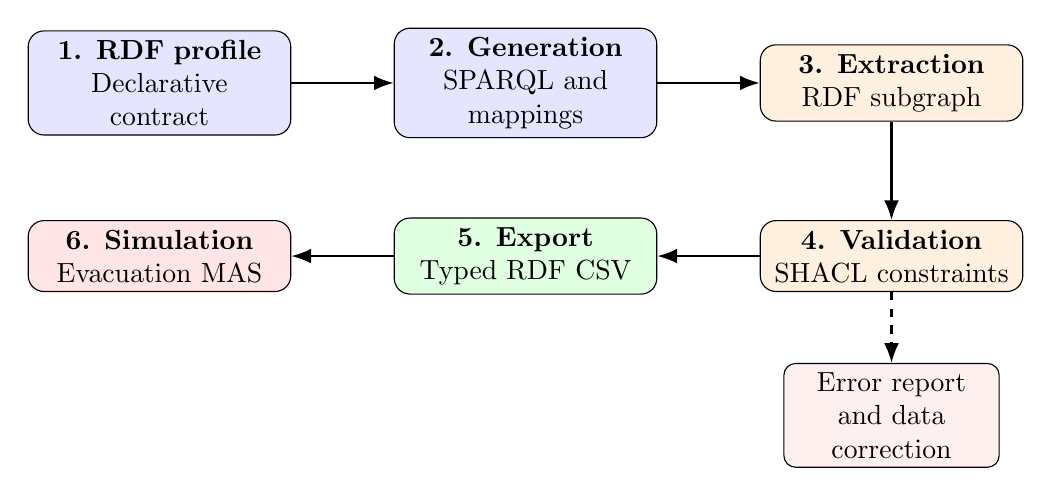
\begin{tikzpicture}[node distance=1.05cm and 1.3cm]
        \node[schemaBox,fill=blue!10] (profile) {\textbf{1. RDF profile}\\Declarative contract};
        \node[schemaBox,fill=blue!10,right=of profile] (queries) {\textbf{2. Generation}\\SPARQL and mappings};
        \node[schemaBox,fill=orange!12,right=of queries] (kg) {\textbf{3. Extraction}\\RDF subgraph};

        \node[schemaBox,fill=orange!12,below=1.25cm of kg] (validation) {\textbf{4. Validation}\\SHACL constraints};
        \node[schemaBox,fill=green!12,left=of validation] (csv) {\textbf{5. Export}\\Typed RDF CSV};
        \node[schemaBox,fill=red!10,left=of csv] (simulation) {\textbf{6. Simulation}\\Evacuation MAS};
        \node[schemaSmall,fill=red!6,below=0.9cm of validation] (errors) {Error report\\and data correction};

        \draw[schemaArrow] (profile) -- (queries);
        \draw[schemaArrow] (queries) -- (kg);
        \draw[schemaArrow] (kg) -- (validation);
        \draw[schemaArrow] (validation) -- (csv);
        \draw[schemaArrow] (csv) -- (simulation);
        \draw[schemaDashed] (validation) -- (errors);
    \end{tikzpicture}
\caption{Preparation and validation of MAS input data}
\label{fig:sma-input-pipeline}
\end{figure}

\begin{filrouge}
\textbf{Preparation of an evacuation of the Bastille} \\
To create a scenario, the graph must link each area of the site to the groups that occupy it and the axes that allow it to leave. The length, width and capacity of these axes are checked prior to simulation. Missing information on a staircase or trail is detected before the MAS calculates trajectories from an incomplete network.
\end{filrouge}

\subsection{Communicating Results and Supporting Decisions}

Communication does not stop at the start of the simulation. The results must return to the graph without losing their production context. The CSV format currently used shall contain at least the identifiers of the execution, scenario, input set and output set, the entity concerned, the stage and simulation time, as well as the property produced, its value and RDF type.

The \texttt{import\_sma\_results\_csv.py} script turns these lines into a \texttt{SPARQL INSERT} query. The values are structured around a simulation run, an output and a final state. They are inserted into a graph dedicated to the results. This separation avoids confusing an observed data with a calculated value in a particular scenario and allows to compare multiple performances.

\begin{lstlisting}[language=SPARQL,caption={Insertion of a simulation result}]
INSERT DATA {
  GRAPH <http://example.org/simulation/results> {
    fe:Run_001 a fe:SimulationRun ;
        fe:usesScenario fe:Scenario_001 ;
        fe:producesOutput fe:Output_001 .

    fe:Output_001 a fe:SimulationOutput ;
        fe:hasFinalState fe:State_Zone_A .

    fe:State_Zone_A a fe:FinalState ;
        fe:stateOfEntity fe:Zone_A ;
        fe:hasSimulationTime 600.0 ;
        fe:hasEvacuationTime 540.0 .
  }
}
\end{lstlisting}

The simulated result is therefore not automatically published as a new current state of the business entity. A calculated fire resistance or accessibility value remains linked to its performance until validated. Publication in the reference graph requires a separate operation, possibly in the form of a \texttt{DELETE/INSERT}, and an explicit updating policy. This precaution is essential for a decision support tool to remain able to explain the origin of information.

The complete chain thus forms a loop whose figure~\ref{fig:simulation-provenance} highlights the links of origin:

\begin{figure}[htbp]
\centering
    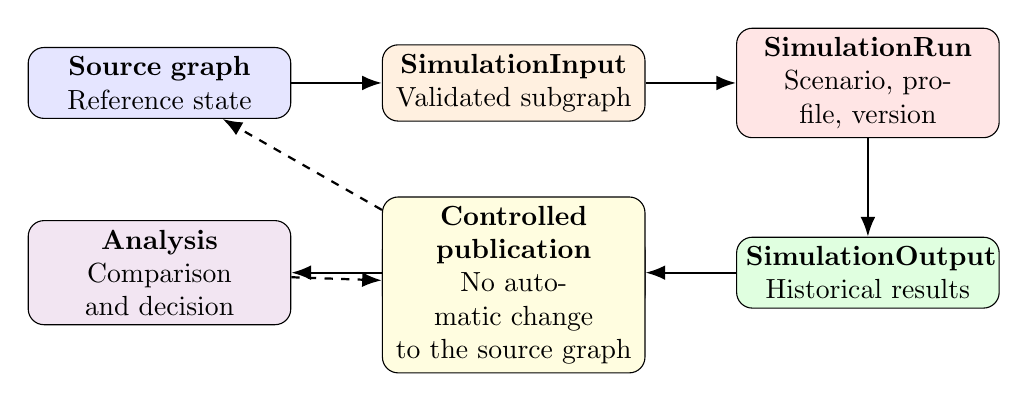
\begin{tikzpicture}[node distance=1.15cm and 1.15cm]
        \node[schemaBox,fill=blue!10] (source) {\textbf{Source graph}\\Reference state};
        \node[schemaBox,fill=orange!12,right=of source] (input) {\textbf{SimulationInput}\\Validated subgraph};
        \node[schemaBox,fill=red!10,right=of input] (run) {\textbf{SimulationRun}\\Scenario, profile, version};

        \node[schemaBox,fill=green!12,below=1.25cm of run] (output) {\textbf{SimulationOutput}\\Historical results};
        \node[schemaBox,fill=green!12,left=of output] (state) {\textbf{FinalState}\\Entity, time, value};
        \node[schemaBox,fill=violet!10,left=of state] (decision) {\textbf{Analysis}\\Comparison and decision};
        \node[schemaBox,fill=yellow!12,below=0.95cm of input] (policy) {\textbf{Controlled publication}\\No automatic change\\to the source graph};

        \draw[schemaArrow] (source) -- (input);
        \draw[schemaArrow] (input) -- (run);
        \draw[schemaArrow] (run) -- (output);
        \draw[schemaArrow] (output) -- (state);
        \draw[schemaArrow] (state) -- (decision);
        \draw[schemaDashed] (decision) -- (policy);
        \draw[schemaDashed] (policy) -- (source);
    \end{tikzpicture}
\caption{Run traceability and separation of source data from simulated results}
\label{fig:simulation-provenance}
\end{figure}

The repository provides generated examples and a series of automated tests. These tests verify the loading of Turtle and SHACL files, the reading of the profile, the stable generation of queries and mappings, the preservation of RDF types during export and the creation of typed SPARQL inserts. They validate the technical chain, but do not replace a scientific evaluation of the behaviour model or real-world experimentation.

The results CSV makes this traceability requirement explicit. Columns \texttt{run\_id}, \texttt{scenario\_id}, \texttt{input\_id}, and \texttt{output\_id} describe the experimental context. Columns \texttt{entity}, \texttt{step}, and \texttt{time} identify the resource and simulation time concerned. Finally, \texttt{property}, \texttt{value}, and \texttt{value\_type} make it possible to reconstruct a correctly typed RDF triple, rather than importing decimal values, Boolean values, and URIs as undifferentiated strings.

The results graph can then be examined from a number of points of view relevant to the decision. A first request compares the evacuation time of the same area between different scenarios. A second identifies the axes whose final state is blocked or whose capacity causes a bottleneck. A third cross-exposed entities, their protection priority and the states produced by the simulation. Ontology does not decide in place of the manager; it organizes the results so that the assumptions and consequences of a recommendation can be traced back.

However, this mechanism has a voluntary limit: the import script produces a layer of snapshots, but does not automatically apply simulated values to reference resources. Such an update would require an assessment of whether the value represents a hypothesis, a prediction at a given moment or a new validated knowledge. The documentation therefore proposes to distinguish an instant retention, an entity update and an associated resource update. This policy will have to be implemented prior to operational use.

\begin{filrouge}
\textbf{Return of Bastille Case Results} \\
If a simulation indicates that a staircase becomes impracticable at the sixth minute, the graph does not permanently replace the accessibility of this staircase. It records that, in a particular scenario and run, a simulated state associates this axis with a blocking at that moment. The manager can then compare this run with a variant in which the start of fire, attendance or opening of an exit differs, without altering the site reference description.
\end{filrouge}

\clearpage
\section{Future Work}
\subsection{Validation Through Real-World Use}

The first perspective is the inskilling of the model on a pilot site with real data. In the case of the Bastille, this stage requires producing or importing the geometry of the zones, the topology of the axes, their dimensions and capacities, the location of buildings and natural spaces, as well as population estimates corresponding to different patterns of use. The correspondence between field data and ontological concepts should be checked with heritage, environmental and simulation specialists.

Validation should operate at several levels. Syntax validation ensures that graphs can be parsed. SHACL checks the completeness required by the use case. Competency queries verify that the graph can answer the questions for which it was designed. Finally, MAS results must be compared with expert scenarios, exercises, or available observations. Semantic conformance alone guarantees neither measurement quality nor behavioural-model validity.

A progressive validation protocol may be envisaged. A first phase would be to collect a static data set limited to a few areas, axes and populations, and then to reread each inskill by field experts. A second phase would introduce several hazard states and verify the profile's ability to produce complete entries. A third phase would compare the outputs of several controlled scenarios. Finally, a site-wide experiment would assess the performance, readability of the results and the real usefulness of requests for decision support.

The evaluation criteria should combine technical and use measures. The rate of compliant data, the number of errors detected before simulation, the reproducibility of exports and the generation time evaluate the computer chain. The ability of experts to retrieve information, understand the origin of a result and specialize in vocabulary evaluates the relevance of the model. On the MAS side, the sensitivity of the results to input data and comparison with baseline scenarios will identify the parameters that require the best quality.

This validation should also consider negative cases. An area without a population, a disconnected axis, a negative capacity, an unknown type or a result without a run ID must produce an understandable failure. The robustness of a decision aid chain depends as much on its ability to reject ambiguous data as on its ability to handle a nominal case.

\subsection{Extension Towards Verification Tools}

One of the ambitions associated with this ontology is ultimately to create a tool for checking data and simulation results. In the field of social simulation, one of the major problems remains the validation of the predictions produced. Collective behaviour is difficult to reproduce experimentally and testing under real-world conditions, particularly when it involves the evacuation of a heritage site exposed to fire, can be costly, difficult to organize or ethically impossible to carry out on a large scale.

The ontology developed in this project provides a first response to this difficulty thanks to the importance attached to traceability. Each simulation can be related to its scenario, input data, parameters used, relevant entities and outputs. The preservation of this information in named graphs helps to preserve the context of each execution without confusing it with the reference data. It then becomes possible to compare a result obtained with an expected result, with another execution of the same model or with data from a previously validated experiment.

From this basis, a verification tool could search the graph for the sites or scenarios closest to the case studied. This proximity would not only be geographical. It could take into account site configuration, the topology and capacity of the axes, population density and composition, the nature of the hazard, weather conditions, the presence of buildings or natural spaces and the parameters of the multi-agent model. The system would thus identify simulations whose entry conditions are sufficiently comparable to constitute relevant reference cases.

The results of a new simulation could then be confronted with those obtained in these comparable cases, with a focus on scenarios where observations, evacuation exercises or experimental validations are available. The objective would not be to automatically demonstrate that a prediction is true, but to assess its plausibility. A large discrepancy with several close cases could indicate an error in input data, a poor scenario configuration, an inconsistency in the behaviour model or, on the contrary, a particular phenomenon requiring scientific analysis. Figure~\ref{fig:simulation-verification} presents the general principle of this comparison.

\begin{figure}[htbp]
\centering
    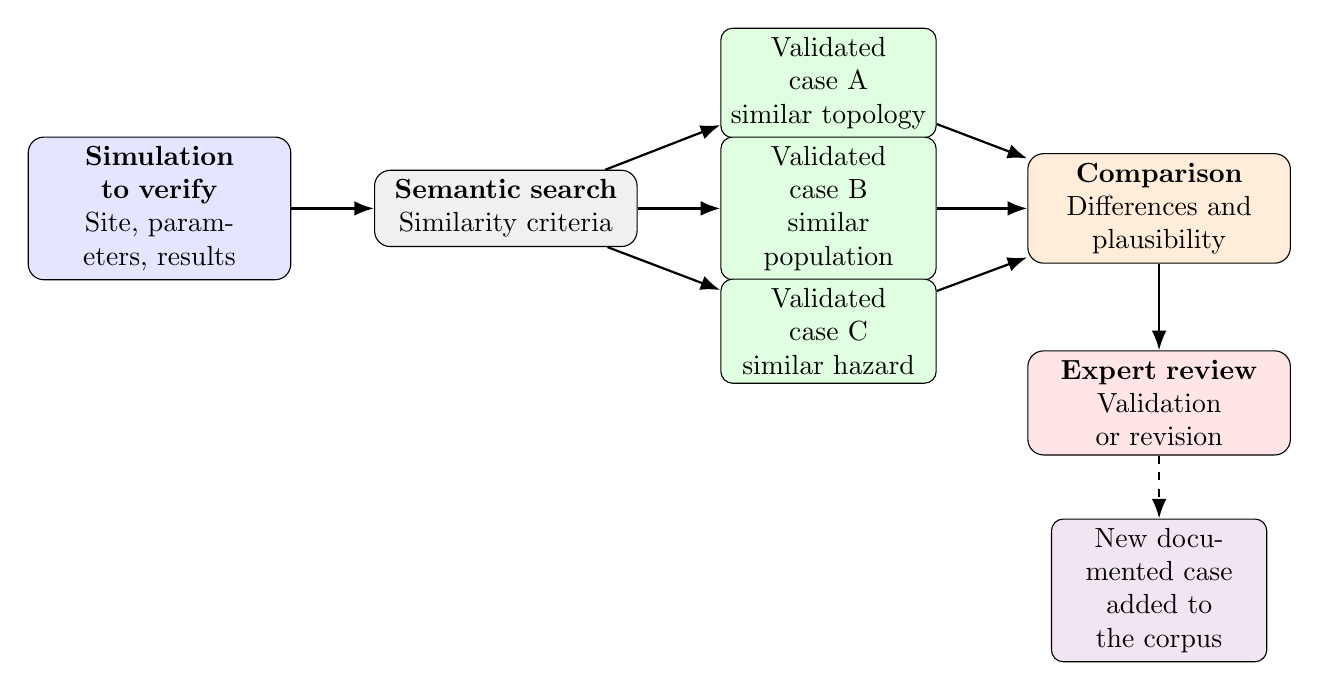
\begin{tikzpicture}[node distance=0.8cm and 1.05cm]
        \node[schemaBox,fill=blue!10] (new) {\textbf{Simulation to verify}\\Site, parameters, results};
        \node[schemaBox,fill=gray!12,right=of new] (search) {\textbf{Semantic search}\\Similarity criteria};

        \node[schemaSmall,fill=green!12,above right=0.4cm and 1.05cm of search] (case1) {Validated case A\\similar topology};
        \node[schemaSmall,fill=green!12,right=1.05cm of search] (case2) {Validated case B\\similar population};
        \node[schemaSmall,fill=green!12,below right=0.4cm and 1.05cm of search] (case3) {Validated case C\\similar hazard};

        \node[schemaBox,fill=orange!15,right=1.15cm of case2] (compare) {\textbf{Comparison}\\Differences and plausibility};
        \node[schemaBox,fill=red!10,below=1.1cm of compare] (review) {\textbf{Expert review}\\Validation or revision};
        \node[schemaSmall,fill=violet!10,below=0.8cm of review] (corpus) {New documented case\\added to the corpus};

        \draw[schemaArrow] (new) -- (search);
        \draw[schemaArrow] (search) -- (case1);
        \draw[schemaArrow] (search) -- (case2);
        \draw[schemaArrow] (search) -- (case3);
        \draw[schemaArrow] (case1) -- (compare);
        \draw[schemaArrow] (case2) -- (compare);
        \draw[schemaArrow] (case3) -- (compare);
        \draw[schemaArrow] (compare) -- (review);
        \draw[schemaDashed] (review) -- (corpus);
    \end{tikzpicture}
\caption{Principle for verifying a simulation against validated cases}
\label{fig:simulation-verification}
\end{figure}

This audit could be based on similar indicators and thresholds defined with experts in the field. Comparisons should remain explicable: the tool should indicate the selected simulations, the parameters considered to be comparable, the observed differences and the criteria leading to an alert. The preservation of inputs and outputs in the graph is essential to this explanation, since it allows the deviation detected to be traced back to the assumptions that produced the result.

Such an extension would gradually transform ontology into an experimental capitalization medium. Each validated simulation would enrich a set of reusable reference cases for the study of new sites. The more documented and validated scenarios the graph would contain, the more the tool would be able to offer relevant comparisons. This approach would not replace human expertise or empirical validation, but would provide a means to monitor the consistency of predictions and detect errors in simulation models sooner.

\subsection{Integration with Platforms Such as ARCH}

Integration with heritage platforms such as ARCH or Arches represents a natural perspective, but it cannot be reduced to importing tables. It requires rules for alignment between identifiers, geometries, asset categories, environmental measures and FE model concepts. CIDOC-CRM provides a first level of interoperability, while specific matches will need to be documented and tested.

In particular, ARCH could provide detailed information on constructions, materials, conservation records and series of measurements. ATLAS ontology would in turn provide a representation adapted to evacuation axes, population groups, operational states and the source of simulations. The aim is therefore not to replace HARIS or THIS, but to establish a semantic pivot allowing their data to feed a multi-agent scenario.

A service interface around a triplestore could eventually automate this stream. The simulator would request an input set corresponding to a profile, only receive validated data, and then file its results in a named graph. This architecture would preserve the essential distinction between heritage reference, observation, scenario hypothesis and simulated value.

Integration requires the definition of explicit correspondence. A HARIS construction must be reconciled with a building class or heritage element; a THIS measurement shall retain its variable, unit, date and provenance; Geometry should be associated with the correct area without confusing administrative location with operational right-of-way. These mappings can be demonstrated by \texttt{CONSTRUCT} queries, correlation tables and, where strong equivalence is warranted, alignment axioms.

Synchronization should also be governed. External platforms will likely remain the authority for certain heritage or environmental data, while the ATLAS graph will be the authority for profiles and simulation results. Setting the source responsible for each information will avoid updating loops and conflicts. Transformations will need to keep the source identifier and import date in order for a data to be verified or refreshed.

This leads to a service architecture rather than a single base absorbing all the others. HARIS, THIS, sensors, triplestore and GAMA can retain their own responsibilities. Ontology then becomes the layer of interoperability that expresses the correspondence, controls the exchange contract and documents the provenance.

\clearpage
\section{Conclusion}
\subsection{Assessment of the Work}

The internship resulted in a deliverable that goes beyond the writing of a vocabulary. Modular ontology covers the main dimensions necessary to describe a heritage site under crisis: spatial organization, construction, circulation, populations, natural environment, weather, hazards, impacts, victims and simulation. Its alignment with CIDOC-CRM maintains a link with heritage standards, while SKOS thesaurus isolate controlled values from the business structure.

The SHACL constraints and the evacuation profile translate the MAS's needs into an inspectionable contract. Generation, export and import scripts make the flow reproducible and tests protect its main technical properties. The separation of simulation results in a historical graph is finally an important contribution to traceability.

However, these results must be evaluated as those of a prototype of research. Full OWL import resolution, automatic shape generation from profiles, direct integration with a triplestore and GAMA and controlled publication of current values are not yet fully automated. The repository demonstrates the architecture and exchange mechanism; it does not yet constitute a system of aid to the decision deployed.

The evaluation can be conducted against the original objectives. Semantic unification is initiated by the core and thematic modules. Heritage interoperability is supported by alignments with CIDOC-CRM and the use of semantic Web standards. The specialisation of values is made possible by SKOS. The input control is materialized by SHACL. Finally, coupling with simulation is demonstrated from end to end on reproducible examples. The result therefore meets the objectives of architecture and prototyping.

However, the objective of an autonomous calculation of vulnerability is only partially achieved. The repository provides the concepts of impact, urgency, state and simulation as well as the mechanisms necessary to extract and reintegrate values, but it does not yet contain a complete catalogue of validated scientific rules calculating all the indices mentioned in the introduction. This distinction is important: the semantic infrastructure is available, while the calculation models will have to be developed and validated with the specialists concerned.

The primary quality of the deliverable is its separation of responsibilities. It allows the evolution of a thesaurus without changing the schema, adding a constraint without transforming an OWL axiom and creating a new profile without rewriting the entire string. Its counterpart is an architecture with several artifacts to maintain consistently. Future audit tools will need to specifically reduce this maintenance cost.

\subsection{Skills and Knowledge Acquired}

This work has deepened the principles of knowledge engineering and measured the difference between the design of a data schema and that of an ontology. RDF/OWL modelling requires reasoning about the identity, scope of relationships, legacy and logical consequences of an axiom. The use of SKOS and SHACL also showed that one language is not enough: representing knowledge, organizing a repository and verifying a requirement are three distinct functions.

The development of the MAS chain has provided additional experience in interoperability. The main difficulty is not only to convert RDF to CSV, but to retain the meaning, type and source when passing between two data paradigms. The drafting of profiles and mappings has led to the formalization of the assumptions that classical interfaces often leave implicit.

Finally, the interdisciplinary nature of the project has reinforced the importance of documentation and examples. An ontology is sustainable only if its choices can be taken up, discussed and specialised by other researchers. Guides, tests and the separation of modules are therefore an integral part of the scientific and technical result.

The approach has also led to a critical posture against standards. Reusing CIDOC-CRM does not mean forcing each operational notion into an existing class; semantically solid alignments should be distinguished from only convenient approximations. Similarly, multiplying classes does not necessarily produce a more precise model. The useful precision results from a compromise between expressivity, understanding by partners and data actually available.

On the software side, the generation of artifacts from a profile showed the value of a declarative design. Automated tests have forced the stabilization of file names, value types and conversion behavior. The recovery documentation finally asked to make explicit decisions previously contained only in Turtle files or scripts.

These learnings are transferable beyond ATLAS: design of a shared model, transformation between graph and table, contextual validation, provenance management and collaboration among specialists from different fields.

\subsection{What Comes Next?}

Beyond the contributions to the ATLAS project, this internship played a key role in defining my professional project. It allowed me to confirm my interest in the engineering and architecture of knowledge, but also in the more fundamental issues of formal representation, logic and inference mechanisms. The design of ontology, its alignment with existing standards and the formalization of exchanges with simulators have shown me that these areas lie precisely at the intersection of my interests in computing, modelling and research.

I now intend to pursue this path by seeking a PhD in knowledge architecture or the formalisation of logical systems. Such a project would allow me to investigate the questions encountered during the internship in greater depth: how to represent heterogeneous knowledge without losing its context, how to verify model consistency, how to combine symbolic reasoning with empirical data, and how to make the results of complex systems explainable. A PhD would provide an opportunity to extend this work within a deeper scientific framework and contribute to the development of new methods.

This research-oriented goal does not exclude entering the profession directly as a knowledge engineer or knowledge architect. The skills acquired during the internship apply to many sectors facing increasing volumes of heterogeneous data: ontology design, knowledge graphs, vocabulary alignment, semantic validation, traceability, and interoperability. I am therefore also interested in industrial or institutional positions where these skills can be applied.

The medical informatics sector is a particularly interesting perspective. Health systems must structure and link data from multiple sources: patient records, medical terminology, biological results, imaging, pharmacopoeia, protein physics, biotechnology, care protocols and research data. Interoperability, data quality and the ability to explain their provenance are key issues. Knowledge architectures can help harmonise this information, monitor its consistency and facilitate its use by both professionals and decision support tools.

So this internship brought me more than just one-off technical experience. It allowed me to identify an area in which it is possible to build the continuation of my career, whether it takes the form of a PhD or a position specialized in knowledge engineering. In both cases, industry and research demonstrate an increasing need to design systems capable of transforming complex and dispersed data into structured, verifiable and truly usable knowledge.

\clearpage
\appendix

\part*{Appendices}
\addcontentsline{toc}{part}{Appendices}
\clearpage

\section{Organisation of the Ontology Deliverable}

This appendix presents the key deliverables directories and their role. It is a quick point of entry for anyone to take over or expand the project.

\begin{description}
\item[\texttt{Ontologies\_KG/Ontologie\_OWL/}] contains the structure of the business model. The \texttt{fe\_core.ttl} file is the entry point and imports the thematic modules.
\item[\texttt{Ontologies\_KG/Thesaurus/}] contains the controlled SKOS vocabularies used to classify entities without multiplying OWL classes.
\item[\texttt{Ontologies\_KG/Constraints/}] brings together the general SHACL and simulation-specific constraints.
\item[\texttt{Ontologies\_KG/Profiles/}] describes the reporting contracts of multi-agent systems, including the evacuation profile.
\item[\texttt{Ontologies\_KG/Request/Templates/}] contains generic SPARQL query templates.
\item[\texttt{Ontologies\_KG/Request/generated/}] brings together reproducible queries, mappings and examples generated from profiles.
\item[\texttt{Ontologies\_KG/Scripts/}] contains programs for generating, exporting entries and importing results.
\item[\texttt{Ontologies\_KG/Tests/}] contains automated tests of the technical chain.
\end{description}

The OWL modules are distributed according to the following responsibilities:

\begin{itemize}
\item \texttt{fe\_site.ttl} and \texttt{fe\_zone.ttl}: spatial organization of sites and study areas;
\item \texttt{fe\_building.ttl}, \texttt{fe\_axis.ttl} and \texttt{fe\_artefacts.ttl}: built environment, traffic and heritage objects;
\item \texttt{fe\_population.ttl}, \texttt{fe\_cognitive\_factor.ttl} and \texttt{fe\_victim.ttl}: populations, behaviours and human consequences;
\item \texttt{fe\_weather.ttl}, \texttt{fe\_natural\_space.ttl}, \texttt{fe\_hazard\_and\_safety.ttl} and \texttt{fe\_hazard\_and\_impact.ttl}: environment, hazards, safety and impacts;
\item \texttt{fe\_simulation.ttl}: scenarios, profiles, executions, inputs, outputs and simulated states.
\end{itemize}

\clearpage
\section{Evacuation MAS Initialisation Profile}

The \texttt{evacuation\_sma\_profile.ttl} profile formalizes the subset of ontology required to initialize the evacuation simulator. The following excerpt presents the essential structure:

\begin{lstlisting}[language=Turtle,caption={Simplified structure of the MAS profile}]
fe:EvacuationSMAProfile a fe:SimulationProfile ;
    fe:profileIdentifier "evacuation_sma" ;
    fe:hasRootClass fe:Zone ;
    fe:requiresClass
        fe:Zone,
        fe:Axis,
        fe:Population,
        fe:HazardEvent ;
    fe:requiresProperty
        fe:hasPopulation,
        fe:isConnectedTo,
        fe:maxFlowCapacity,
        fe:hasWidth,
        fe:hasLength,
        fe:hasEstimatedCount,
        fe:hasHazardType,
        fe:hasHazardExposure ;
    fe:optionalProperty
        fe:containsBuilding,
        fe:containsNaturalSpace,
        fe:hasWeatherCondition,
        fe:hasBlockingState ;
    fe:producesClass
        fe:SimulationOutput,
        fe:FinalState,
        fe:StateSnapshot .
\end{lstlisting}

Profile predicates have distinct functions:

\begin{description}
\item[\texttt{fe:hasRootClass}] defines the conceptual entry point for extraction.
\item[\texttt{fe:requiresClass}] refers to the categories of entities that the MAS must be able to receive.
\item[\texttt{fe:requiresProperty}] declares the information necessary for calculation.
\item[\texttt{fe:optionalProperty}] declares the information able to enrich the scenario without blocking its initialization.
\item[\texttt{fe:producesClass}] and \texttt{fe:producesProperty} document the nature of the expected results.
\end{description}

The generator extracts the required and optional properties flexibly. Their mandatory nature is controlled separately by SHACL. This distinction keeps an open RDF graph while imposing a stricter contract at the time of simulation.

\clearpage
\section{Generation and Data-Exchange Workflow}

The following commands are executed from the repository root. They assume the prior installation of the dependencies reported in \texttt{requirements.txt}.

\subsection{Installation and Tests}

\begin{lstlisting}
python -m pip install -r requirements.txt

python -m unittest discover \
  -s Ontologies_KG/Tests -v
\end{lstlisting}

\subsection{Generating Queries and Mappings}

\begin{lstlisting}
python Ontologies_KG/Scripts/generate_sma_queries.py \
  Ontologies_KG/Profiles/evacuation_sma_profile.ttl \
  --out-dir Ontologies_KG/Request/generated \
  --template-dir Ontologies_KG/Request/Templates
\end{lstlisting}

This command includes \texttt{CONSTRUCT} and \texttt{SELECT} initialization requests, the result insertion model and JSON files describing the matches.

\subsection{Exporting Input Data}

\begin{lstlisting}
python Ontologies_KG/Scripts/export_sma_input_csv.py \
  --profile Ontologies_KG/Profiles/evacuation_sma_profile.ttl \
  --data chemin/vers/kg.ttl \
  --out exports/evacuation_sma_input.csv
\end{lstlisting}

The input CSV follows the following structure:

\begin{lstlisting}
entity,class,property,value,value_type,value_lang
fe:Axis_12,fe:Axis,fe:maxFlowCapacity,150,xsd:integer,
fe:Axis_12,fe:Axis,fe:hasWidth,3.5,xsd:double,
\end{lstlisting}

\subsection{SHACL Validation}

\begin{lstlisting}
pyshacl \
  -s Ontologies_KG/Constraints/evacuation_sma_input_shape.ttl \
  -d Ontologies_KG/Request/generated/evacuation_sma_sample_data.ttl \
  -f human
\end{lstlisting}

\texttt{Conforms: True} indicates that the graph meets the minimum requirements of the profile. In the event of failure, the report shall refer to the resource concerned, the missing or incorrect property and the message associated with the constraint.

\subsection{Importing Results}

\begin{lstlisting}
python Ontologies_KG/Scripts/import_sma_results_csv.py \
  --profile Ontologies_KG/Profiles/evacuation_sma_profile.ttl \
  --csv exports/evacuation_sma_results.csv \
  --out Ontologies_KG/Request/generated/results_insert.sparql
\end{lstlisting}

The resulting SPARQL file inserts the results into a graph named separate from the source graph. This operation preserves the history of the run without automatically replacing the current state of the business entities.

\clearpage
\section{Simulation-Result Contract}

The results CSV shall contain at least the following columns:

\begin{lstlisting}
run_id,scenario_id,input_id,output_id,entity,step,time,
property,value,value_type
\end{lstlisting}

\begin{description}
\item[\texttt{run\_id}] identifies the actual execution of the simulator.
\item[\texttt{scenario\_id}] identifies the hypothesis or configuration studied.
\item[\texttt{input\_id}] is the data set used for initialization.
\item[\texttt{output\_id}] identifies the product result lot.
\item[\texttt{entity}] retains the identifier of the relevant business resource.
\item[\texttt{step} and \texttt{time}] place the value in simulated time.
\item[\texttt{property}] indicates the RDF predicate associated with the result.
\item[\texttt{value}] contains the value produced by the MAS.
\item[\texttt{value\_type}] specifies whether it is a URI or a typed literal.
\end{description}

Example of results:

\begin{lstlisting}
run_id,scenario_id,input_id,output_id,entity,step,time,
property,value,value_type
SimulationRun_001,Scenario_001,Input_evacuation_sma,
Output_001,Zone_A,120,600.0,fe:hasFinalStatus,
evacuated,xsd:string
SimulationRun_001,Scenario_001,Input_evacuation_sma,
Output_001,Zone_A,120,600.0,fe:hasEvacuationTime,
540.0,xsd:double
\end{lstlisting}

The import creates instances of \texttt{fe:SimulationRun}, \texttt{fe:SimulationOutput} and \texttt{fe:FinalState}. The source links allow to find the scenario and the input game that produced each value. A direct update of the source entity must remain a separate and explicitly validated operation.

\clearpage
\section{Specialisation Checklist}

When a researcher wishes to expand the deliverable, the recommended procedure is:

\begin{enumerate}
\item identify the OWL module responsible for the concept;
\item check whether the concept should be a structured class or a SKOS concept;
\item reuse a CIDOC-CRM class when a relevant semantic alignment exists;
\item define classes and properties with appropriate wording, comment, domain and range;
\item add the controlled values in the corresponding thesaurus;
\item complete SHACL constraints if data becomes mandatory;
\item update the SMA profile if the property is consumed or produced by the simulator;
\item regenerate requests, mappings and examples;
\item perform automated tests and validate sample data;
\item document the need for the amendment.
\end{enumerate}

This procedure maintains the separation between domain structure, terminology, data quality and application contract. It also reduces the risk that a specific simulator requirement will be imposed on the entire ontology.

\end{document}
